% TODO: -

%%%%%%%%%%%%%%%%%%%%%%%
% Dokument definieren %
%%%%%%%%%%%%%%%%%%%%%%%

\documentclass[a4paper, 12pt]{article}

%%%%%%%%%%%%%%%%%%%%%%%%%%%%%%%%%%
% Pakete laden und konfigurieren %
%%%%%%%%%%%%%%%%%%%%%%%%%%%%%%%%%%

% deutsche Spracheinstellungen und -kodierung
\usepackage[utf8]{inputenc}                                                 % Umlaute korrekt verwenden
\usepackage[T1]{fontenc}                                                    % Schriftenkodierung
\usepackage[ngerman]{babel}                                                 % Deutsche Spracheinstellungen
\usepackage{csquotes}                                                       % Für korrekte Anführungszeichen
\usepackage{hyphenat}                                                       % Silbentrennung

% Pakete für R
\usepackage{tabularray}                                                     % Für erweiterte Tabellen
\usepackage{float}                                                          % Fixiert Objekte mit "H"
\usepackage[normalem]{ulem}                                                 % Für Unter- und Durchstreichungen
\UseTblrLibrary{booktabs}                                                   % Unterstützt Booktabs in Tabellen
\UseTblrLibrary{siunitx}                                                    % Unterstützt Zahlen und Einheiten
\newcommand{\tinytableTabularrayUnderline}[1]{\underline{#1}}               % Unterstreichung in Tabellen
\newcommand{\tinytableTabularrayStrikeout}[1]{\sout{#1}}                    % Durchstreichung in Tabellen
\NewTableCommand{\tinytableDefineColor}[3]{\definecolor{#1}{#2}{#3}}        % Farben in Tabellen
\usepackage{adjustbox}                                                      % Skaliert Tabellen/Objekte
\usepackage{multicol}                                                       % Mehrspaltiger Text
\usepackage{listings}                                                       % Für Code-Listings
\lstset{
    language=R,                                                             % Specify the language
    basicstyle=\ttfamily\scriptsize,                                        % Font style for code
    numbers=left,                                                           % Line numbers on the left
    numberstyle=\tiny,                                                      % Font size for line numbers
    stepnumber=1,                                                           % Number every line
    breaklines=true,                                                        % Automatically break long lines
    frame=single,                                                           % Add a border around the code
    captionpos=b,                                                           % Caption position (bottom)
    showstringspaces=false                                                  % Do not show spaces in strings
}

% Layout und Seitenränder
\usepackage{geometry}
\geometry{a4paper, top=3cm, bottom=3cm, left=2.5cm, right=2.5cm}

% Literaturverzeichnis mit APA-Zitierstil
\usepackage[style=apa, backend=biber, language=ngerman]{biblatex}
\addbibresource{assets/literature.bib}                                      % Bibliographiedatei einbinden

% Pakete für Abkürzungsverzeichnis und Glossar
\usepackage[printonlyused]{acronym}

% mathematische Symbole (optional)
\usepackage{amsmath, amssymb}

% Für Tabellen und Grafiken
\usepackage{graphicx}                                                       % Für Bilder
\usepackage{booktabs}                                                       % Für schönere Tabellen

% Hyperlinks
\usepackage[hidelinks]{hyperref}

% Codebook einbinden
\usepackage{verbatim}                                                       % Für Einbinden als plain text

% Zeilenabstand
\usepackage{setspace}
\onehalfspacing                                                             % 1,5-facher Zeilenabstand

% Kopf- und Fußzeilen
\usepackage{fancyhdr}
\pagestyle{fancy}
\fancyhf{}                                                                  % Setzt Kopf- und Fußzeile zurück
\fancyhead[R]{T. A. Rau}                                                    % Name links
\fancyhead[L]{ICT-Investitionen und Arbeitslosigkeit in Wohlfahrtsstaaten}  % Titel rechts
\setlength{\headheight}{14.5pt}                                             % Setzt die Höhe der Kopfzeile
\fancyfoot[C]{\thepage}                                                     % Setzt die Seitenzahl mittig unten

%%%%%%%%%%%%%%%%%%%%%
% Dokument beginnen %
%%%%%%%%%%%%%%%%%%%%%

% Titel und Autoreninformationen
\title{ICT-Investitionen und Arbeitslosigkeit in Wohlfahrtsstaaten\\ 
\large Eine Paneldatenanalyse nach Bildungsniveau in OECD-Ländern}
\author{Tobias Achim Rau}
\date{\today}

\begin{document}

% Titelseite
\maketitle
\thispagestyle{empty}
\vspace{2cm}

\begin{center}
  \textbf{Bachelorarbeit} \\
  vorgelegt im Studiengang Politikwissenschaften \\
  am Fachbereich 03 an der \textbf{Goethe-Universität Frankfurt} \\
  \vspace{2cm}
  \textbf{Verfasser:} Tobias Achim Rau \\
  \textbf{Matrikelnummer:} 6619097 \\
  \textbf{E-Mail:} s3045892@stud.uni-frankfurt.de \\
  \vspace{2cm}
  \textbf{Betreuerin:} Anna Gerlach \\
  \vspace{2cm}
  \textbf{Abgabedatum:} 25.03.2025
\end{center}

\newpage

% Inhaltsverzeichnis
\tableofcontents

\newpage

% Abkürzungsverzeichnis
\section*{Abkürzungsverzeichnis}
\begin{acronym}[SNA08] % Breite der längsten Abkürzung für Ausrichtung
  \acro{ICT}{Informations- und Kommunikationstechnologien (aus d. Engl.: 
  \textit{Information and Communication Technologies})}
  
  \acro{OECD}{Organisation für wirtschaftliche Zusammenarbeit und Entwicklung 
  (aus d. Engl.: \textit{Organisation for Economic Co-operation and Development})}
 
  \acro{SNA08}{System of National Accounts 2008}

  \acro{SBTC}{Skill-Biased Technological Change (z. Dt.: \textit{Technologie mit 
  qualifikationsspezifischen Effekten})}

  \acro{RBTC}{Routine-Biased Technological Change (z. Dt.: \textit{Technologie mit 
  routinespezifischen Effekten})}
  
  \acro{BIP}{Bruttoinlandsprodukt}
  
  \acro{RE}{Random Effects (z. Dt.: \textit{zufällige Effekte})}
  
  \acro{FE}{Fixed Effects (z. Dt.: \textit{feste Effekte})}

  \acro{AI}{Künstliche Intelligenz (aus d. Engl.: \textit{Artificial Intelligence})}

  \acro{IoT}{Internet der Dinge (aus d. Engl.: \textit{Internet of Things})}
\end{acronym}

\newpage

% Glossar
\section*{Glossar}
\begin{description}
  \item[Digitalisierung] bezeichnet den Prozess der Umwandlung von analogen Informationen, 
  Prozessen und Geschäftsmodellen in digitale Formate. Sie umfasst den Einsatz digitaler 
  Technologien zur Automatisierung und Optimierung von Abläufen sowie zur Schaffung neuer 
  Wertschöpfungspotenziale \parencite[S. 6]{brennen2016theinternational}. Im 
  wirtschaftlichen Kontext wird Digitalisierung oft im Zusammenhang mit der vierten 
  industriellen Revolution (Industrie 4.0) gesehen, die durch die Integration digitaler 
  und physischer Systeme gekennzeichnet ist \parencite[S. 114]{hofman2018arbeit}.

  \item[Cloud Computing] beschreibt die Bereitstellung von IT-Ressourcen wie Speicherplatz, 
  Rechenleistung und Anwendungen über das Internet („die Cloud“) anstelle lokaler Server 
  oder Computer. Dieses Modell ermöglicht den flexiblen Zugriff auf Daten und Anwendungen 
  unabhängig vom Standort und fördert Skalierbarkeit sowie Kosteneffizienz 
  \parencite[S. 52]{armbrust2010aview}. Die wichtigsten Servicemodelle sind 
  Infrastructure-as-a-Service, Platform-as-a-Service und 
  Software-as-a-Service.

  \item[Künstliche Intelligenz] bezeichnet die Fähigkeit von Maschinen oder 
  Computersystemen, menschenähnliche kognitive Funktionen wie Lernen, Problemlösung und 
  Entscheidungsfindung auszuführen. Sie basiert auf Algorithmen, die Muster in Daten 
  erkennen und selbstständig aus Erfahrungen lernen können 
  \parencite[S. 28]{russell2020artificial}. \ac{AI} umfasst verschiedene Teilbereiche wie 
  maschinelles Lernen, neuronale Netzwerke und natürliche Sprachverarbeitung.

  \item[Big Data] bezeichnet große, komplexe und schnell wachsende Datenmengen, die mit 
  herkömmlichen Datenverarbeitungssystemen nur schwer analysierbar sind. Die Analyse 
  von Big Data erfolgt häufig mit Verfahren des maschinellen Lernens, Data Mining und 
  verteilten Datenbanksystemen \parencite[S. 92]{gandomi2014beyond}.

  \item[Reversed Causality] beschreibt eine umgekehrte Kausalbeziehung zwischen zwei Variablen, 
  bei der die vermeintliche unabhängige Variable tatsächlich durch die abhängige Variable 
  beeinflusst wird. Dies kann zu Fehlinterpretationen in statistischen Analysen führen, 
  insbesondere in nicht-experimentellen Studien. Reversed Causality tritt häufig in 
  wirtschaftlichen und sozialwissenschaftlichen Untersuchungen auf 
  \parencite[S. 134]{pearl2009causality}.
\end{description}

\newpage

% Kapitel einbinden
% TODO: Keine TODOs.

\section{Einleitung}

Mit der zunehmenden Digitalisierung und Automatisierung der Arbeitswelt erleben viele 
Länder tiefgreifende strukturelle Veränderungen ihrer Arbeitsmärkte. Eine zentrale Rolle 
spielen dabei \ac{ICT}, deren Einsatz weltweit zu erheblichen Effizienzsteigerungen und 
Innovationsprozessen führt \parencite[vgl.][S. 90–93]{brynjolfsson2015thesecond}.

Während technologische Fortschritte die Nachfrage nach hochqualifizierten Arbeitskräften 
erhöhen können, bleibt unklar, welche Auswirkungen diese Entwicklung auf 
geringqualifizierte Arbeitskräfte hat und inwiefern sie sich messen lässt 
\parencite[vgl.][S. 1045]{acemoglu2011skills}. Einerseits eröffnen die gestiegenen 
Anforderungen an technologische Kompetenzen neue Chancen für hochqualifizierte Fachkräfte 
\parencite[vgl.][S. 1070]{acemoglu2011skills}, andererseits wächst die Befürchtung, dass 
rasante Investitionen in \ac{ICT} den Zugang zu Arbeitsplätzen für geringqualifizierte 
Personen erschweren \parencite[vgl.][S. 14-15]{frey2013thefuture}. In der Forschung wird 
daher diskutiert, ob der technologische Fortschritt die Kluft zwischen den 
Bildungsniveaus weiter vertieft und die Arbeitslosigkeit unter geringer 
Qualifizierten verstärkt \parencite[vgl.][S. 2–4]{balsmeier2019isthis}.

Die Frage nach dem Zusammenhang zwischen \ac{ICT}-Investitionen und Arbeitslosigkeit 
nach Bildungsniveau ist nicht nur ökonomisch, sondern auch sozial von Bedeutung. 
Investitionen in digitale Technologien können Polarisierungseffekte hervorrufen, 
indem sie hochqualifizierte Arbeitskräfte begünstigen, während geringer Qualifizierte 
durch Automatisierung verdrängt werden \parencite[vgl.][S. 14–15]{frey2013thefuture}. 
Gleichzeitig entstehen durch den technologischen Wandel neue Berufsfelder, die 
innovative Fähigkeiten erfordern \parencite[vgl.][S. 3–6]{brynjolfsson2015thesecond}. 
Welche Auswirkungen diese Prozesse auf die Verteilung von Arbeitsplätzen haben und 
ob sie zur Polarisierung des Arbeitsmarktes beitragen, bleibt eine zentrale Frage der 
aktuellen Forschung \parencite[vgl.][S. 2–4]{balsmeier2019isthis}.

Ziel dieser Arbeit ist es daher, den Einfluss von \ac{ICT}-Investitionen auf die 
Arbeitslosigkeit in verschiedenen Bildungsgruppen zu untersuchen. Es wird angenommen, 
dass hohe Investitionen in digitale Technologien die Arbeitslosigkeit unter 
Hochqualifizierten senken, während sie bei geringer Qualifizierten steigen könnte 
\parencite[vgl.][S. 1045]{acemoglu2011skills}. Diese Analyse soll zur Debatte über die 
Folgen der Digitalisierung auf den Arbeitsmarkt beitragen und empirisch untersuchen, 
in welchem Maße technologische Investitionen mit der Arbeitslosenquote nach 
Bildungsniveau korrelieren.

Aus der zuvor dargelegten Argumentation ergibt sich die zentrale Forschungsfrage 
dieser Arbeit:

\begin{quote} \textbf{„Wie beeinflussen nationale Investitionen in Informations- und 
    Kommunikationstechnologien die Arbeitslosenquoten verschiedener Bildungsniveaus 
    in Wohlfahrtsstaaten?“} \end{quote}

Die Analyse der Auswirkungen von Digitalisierung und \ac{ICT}-Investitionen auf die 
Beschäftigungsstruktur in \ac{OECD}-Ländern ist von hoher Relevanz, da sie Aufschluss 
über die Anpassungsfähigkeit verschiedener Wirtschaftssysteme an technologische 
Umbrüche gibt. Zudem bietet sie eine Grundlage für politische Entscheidungen im 
Bereich Arbeitsmarktregulierung und Bildungsinvestitionen. Angesichts der zunehmenden 
Bedeutung digitaler Technologien für wirtschaftliches Wachstum und soziale 
Gerechtigkeit ist es essenziell, die damit verbundenen Herausforderungen und Chancen 
für verschiedene gesellschaftliche Gruppen besser zu verstehen.

% TODO: - (Passt so.)

\section{Forschungsgegenstand}

Der Forschungsgegenstand dieser Arbeit umfasst die Untersuchung der Auswirkungen von 
Investitionen in \ac{ICT} auf den Arbeitsmarkt in \ac{OECD}-Ländern. Im Zentrum steht 
dabei die Frage, wie sich diese Investitionen auf die Beschäftigungslage, insbesondere 
die Arbeitslosenquote, in verschiedenen Bildungsgruppen auswirken. Dabei werden sowohl 
die nationalen Investitionen in digitale Technologien als auch die Auswirkungen auf 
Arbeitsmärkte und Beschäftigungsstrukturen betrachtet.

%%%%%%%%%%%%%%%%%%%%%%%%%%%%%%%%%%%%%
% Digitalisierung und Industrie 4.0 %
%%%%%%%%%%%%%%%%%%%%%%%%%%%%%%%%%%%%%

\subsection{Digitalisierung und Industrie 4.0}

Der Begriff der Digitalisierung beschreibt den zunehmenden Einsatz digitaler Technologien 
zur Automatisierung, Optimierung und Schaffung neuer Wertschöpfungspotenziale 
\parencite[vgl.][S. 6]{brennen2016theinternational}. Im wirtschaftlichen Kontext wird dies 
mit der vierten industriellen Revolution (Industrie 4.0) in Verbindung gebracht, die durch 
die Integration von \ac{ICT}, \ac{AI}, Big Data, Cloud Computing, Cyber-Physischen Systemen 
sowie dem \ac{IoT} gekennzeichnet ist \parencite[vgl.][S. 22]{kagermann2013recommendations}. 
Diese technologischen Fortschritte ermöglichen eine umfassende Automatisierung von 
Produktionsabläufen und eine Vernetzung einzelner Prozessschritte. Unternehmen profitieren 
durch höhere Effizienz, geringere Produktionskosten und eine flexiblere Fertigung. Ein 
zentraler Faktor ist die Möglichkeit, Daten in Echtzeit zu erfassen, zu analysieren und 
zur Prozessoptimierung zu nutzen, beispielsweise durch „vorausschauende Wartung“ 
(\textit{predictive maintenance}), wodurch Maschinenausfälle minimiert werden 
\parencite[vgl.][S. 85]{bartodziej2016theconcept}. 

Der Wandel durch Industrie 4.0 hat weitreichende Implikationen für den Arbeitsmarkt. 
Einerseits entstehen neue hochqualifizierte Arbeitsplätze in den Bereichen 
Softwareentwicklung, Datenanalyse und Automatisierungstechnik. Andererseits führt die 
Digitalisierung in vielen Sektoren zur Verdrängung traditioneller Routinetätigkeiten, 
insbesondere in der industriellen Fertigung, im Transportwesen und in administrativen 
Berufen \parencite[vgl.][S. 40]{frey2013thefuture}. Dadurch entstehen signifikante 
Unterschiede in der Betroffenheit verschiedener Bildungsgruppen vom technologischen Wandel. 
Zudem verändert sich die Arbeitsorganisation durch flexible Arbeitszeitmodelle, Remote 
Work und Plattformarbeit \parencite[vgl.][S. 112]{schwab2016thefourth}. Die digitale 
Vernetzung erfordert neue Kompetenzen und Anpassungsstrategien für Arbeitnehmer*innen, 
während gleichzeitig Fragen zu Datenschutz, IT-Sicherheit und algorithmengesteuerten 
Entscheidungsprozessen an Bedeutung gewinnen.

%%%%%%%%%%%%%%%%%%%%%
% ICT-Investitionen %
%%%%%%%%%%%%%%%%%%%%%

\subsection{ICT-Investitionen}

Investitionen in \ac{ICT} umfassen materielle und immaterielle Ressourcen, die zur 
Digitalisierung von Wirtschaft und Gesellschaft beitragen. Dazu zählen physische 
Infrastrukturen wie Glasfasernetze und Rechenzentren sowie immaterielle Investitionen in 
Software, Cloud-Dienste und digitale Plattformen 
\parencite[vgl.][S. 15ff]{oecd2019measuring}. Sie sind ein wesentlicher Indikator für die 
digitale Transformation eines Landes und beeinflussen maßgeblich die Integration neuer 
Technologien in Produktions- und Dienstleistungsprozesse.

Der verstärkte Einsatz digitaler Technologien ermöglicht nicht nur Effizienzsteigerungen, 
sondern auch die Entwicklung neuer Geschäftsmodelle. Fortschritte in \ac{AI} und Big Data 
führen zur Automatisierung vieler Prozesse, wodurch Unternehmen flexibler auf 
Marktentwicklungen reagieren können \parencite[vgl.][S. 15ff]{oecd2019measuring}. 
Gleichzeitig erlaubt der Einsatz von \ac{AI} eine effizientere Datennutzung, wodurch 
Entscheidungsprozesse optimiert werden.

\ac{ICT}-Investitionen sind zudem ein Schlüsselfaktor für wirtschaftliches Wachstum. 
Studien zeigen eine positive Korrelation zwischen Digitalisierung, Innovationsfähigkeit 
und der Wettbewerbsfähigkeit von Unternehmen 
\parencite[vgl.][S. 22]{brynjolfsson2014thesecond}. Besonders in digital führenden Ländern 
wie den USA oder Deutschland sind diese Investitionen ein Treiber von 
Produktivitätssteigerungen. Gleichzeitig können sie dazu beitragen, strukturelle 
Ungleichheiten zwischen urbanen und ländlichen Regionen zu verringern.

Allerdings sind die Auswirkungen von \ac{ICT}-Investitionen auf den Arbeitsmarkt 
ambivalent. Während neue Arbeitsplätze in zukunftsorientierten Bereichen entstehen, führt 
die Automatisierung gleichzeitig zur Substitution von Routinetätigkeiten, insbesondere 
bei Berufen mit mittlerem Qualifikationsniveau \parencite[vgl.][S. 40]{frey2013thefuture}. 
Dies verstärkt bestehende Arbeitsmarktungleichheiten.

%%%%%%%%%%%%%%%%%%%%%%%%%%%%%
% Arbeitsmarkt und Bildung %
%%%%%%%%%%%%%%%%%%%%%%%%%%%%%

\subsection{Arbeitsmarkt und Bildungsgruppen}

Der Arbeitsmarkt ist geprägt durch strukturelle Veränderungen infolge technologischer 
Innovationen. In dieser Arbeit liegt der Fokus auf der Arbeitslosigkeit nach 
Bildungsniveau, die üblicherweise in niedrig, mittel und hoch eingeteilt wird 
\parencite[vgl.][S. 35–37]{frey2013thefuture}. Diese Differenzierung ermöglicht eine 
gezielte Analyse der Betroffenheit unterschiedlicher Gruppen.

Die Auswirkungen der Digitalisierung auf den Arbeitsmarkt werden häufig mit dem Konzept 
der Jobpolarisierung beschrieben. Hochqualifizierte Fachkräfte profitieren von der 
steigenden Nachfrage nach digitalen Kompetenzen, während Arbeitsplätze mit mittleren 
Qualifikationsanforderungen verstärkt unter Automatisierungsdruck geraten 
\parencite[vgl.][S. 40]{autor2015whyare}. Geringqualifizierte sind besonders anfällig für 
Arbeitsplatzverdrängung, da ihre Tätigkeiten häufig leicht durch technologische Systeme 
ersetzt werden können \parencite[vgl.][S. 10]{acemoglu2002technical}.

Frey und Osborne (2013) schätzen, dass rund 47~\% der Arbeitsplätze in den USA potenziell 
automatisierbar sind, wobei insbesondere Berufe mit niedriger Qualifikation betroffen sind 
\parencite[vgl.][S. 14–15]{frey2013thefuture}. In der Forschung wird daher diskutiert, ob 
technologischer Fortschritt die Kluft zwischen den Bildungsniveaus weiter vertieft und die 
Arbeitslosigkeit unter geringer Qualifizierten verstärkt 
\parencite[vgl.][S. 2–4]{balsmeier2019isthis}. Um den negativen Effekten entgegenzuwirken, 
werden gezielte bildungs- und arbeitsmarktpolitische Maßnahmen als notwendig erachtet. 
Besonders Weiterbildungsprogramme für digitale Kompetenzen sind zentral, um den 
Strukturwandel am Arbeitsmarkt abzufedern \parencite[vgl.][S. 75]{brynjolfsson2014thesecond}. 
Länder mit einem gut ausgebauten Weiterbildungssystem können die negativen Folgen der 
Arbeitsmarktpolarisierung besser kompensieren.

Zusammenfassend hängt der Einfluss von \ac{ICT}-Investitionen auf den Arbeitsmarkt stark 
vom Bildungsniveau der Erwerbsbevölkerung ab. Während Hochqualifizierte profitieren, 
sehen sich niedrig und mittel qualifizierte Arbeitskräfte mit zunehmender Unsicherheit 
konfrontiert. Diese Entwicklung verdeutlicht die Notwendigkeit einer gezielten 
politischen Steuerung, um sozial-ökonomische Risiken zu minimieren.

% TODO: - (Passt so.)

\section{Forschungsstand}

Die Auswirkungen von Digitalisierung und \ac{ICT}-Investitionen auf den Arbeitsmarkt sind 
ein zentrales Thema der arbeitsmarktökonomischen Forschung. Während einige Studien den 
Fokus auf die technologische Verdrängung bestimmter Berufsgruppen legen, untersuchen 
andere, inwieweit institutionelle Rahmenbedingungen wie Wohlfahrtsstaaten die Effekte von 
Digitalisierung abmildern oder verstärken. In diesem Kapitel werden zunächst die 
allgemeinen Auswirkungen der Digitalisierung auf Arbeitsmärkte analysiert, bevor der Fokus 
auf die Rolle von \ac{ICT}-Investitionen und die Unterschiede zwischen verschiedenen 
Wohlfahrtsstaaten gelegt wird. Abschließend werden bestehende Forschungslücken aufgezeigt, 
die eine weiterführende Analyse notwendig machen.

%%%%%%%%%%%%%%%%%%%%%%%%%%%%%%%%%%%%%%%%%%%%%%%%%%%%%%
% Auswirkungen der Digitalisierung auf Arbeitsmärkte %
%%%%%%%%%%%%%%%%%%%%%%%%%%%%%%%%%%%%%%%%%%%%%%%%%%%%%%

\subsection{Auswirkungen der Digitalisierung auf Arbeitsmärkte}

Die Digitalisierung und insbesondere Investitionen in \ac{ICT} haben die Arbeitsmärkte 
weltweit in den letzten Jahrzehnten grundlegend verändert. Empirische Studien zeigen, dass 
diese Entwicklungen die Beschäftigungsstrukturen in verschiedenen Bildungsgruppen 
unterschiedlich beeinflussen \parencite[vgl.][S. 7]{autor2013thegrowth}. Die Automatisierung 
technologischer Prozesse sowie der verstärkte Einsatz digitaler Systeme betreffen 
insbesondere Tätigkeiten, die routinisierbar und standardisierbar sind 
\parencite[vgl.][S. 20]{frey2013thefuture}. In diesem Zusammenhang haben verschiedene 
wissenschaftliche Arbeiten untersucht, welche Beschäftigungsgruppen besonders von den 
digitalen Transformationsprozessen betroffen sind.

Eine der einflussreichsten Arbeiten in diesem Bereich stammt von Autor, Levy und Murnane 
(2003), die zeigen, dass Tätigkeiten mit einem hohen Anteil an routinemäßigen kognitiven 
und manuellen Aufgaben besonders anfällig für Automatisierung sind. Die daraus resultierende 
Theorie des \ac{RBTC} besagt, dass Digitalisierung insbesondere Arbeitsplätze betrifft, die 
in klar definierten, sich wiederholenden Mustern ablaufen und daher relativ leicht durch 
Algorithmen und Maschinen ersetzt werden können \parencite[vgl.][S. 1281]{autor2003theskill}. 
Frey und Osborne (2017) erweiterten diese Analyse und quantifizierten das 
Substitutionsrisiko durch Automatisierung für verschiedene Berufsgruppen. Ihre 
Untersuchung für den US-amerikanischen Arbeitsmarkt ergab, dass bis zu 47\% der 
Arbeitsplätze potenziell durch Automatisierung ersetzt werden könnten 
\parencite[vgl.][S. 254]{frey2013thefuture}. Dabei stellten sie fest, dass vor allem Berufe mit 
niedrigem Qualifikationsniveau gefährdet sind, insbesondere in den Bereichen administrative 
Tätigkeiten, einfache Produktionstätigkeiten und Transportwesen. Diese Ergebnisse sind auch 
auf viele \ac{OECD}-Länder übertragbar, da ähnliche Beschäftigungsstrukturen und 
Automatisierungstrends in entwickelten Volkswirtschaften zu beobachten sind.

Parallel zur Automatisierung zeigt sich eine Polarisierung der Arbeitsmärkte, die von Goos, 
Manning und Salomons (2014) ausführlich analysiert wurde. Ihre Untersuchung belegt, dass die 
Digitalisierung gleichzeitig Berufe stärkt, die komplexe kognitive, kreative oder soziale 
Fähigkeiten erfordern \parencite[vgl.][S. 2509]{goos2014explaining}. Während mittlere 
Qualifikationsgruppen unter Druck geraten, profitieren insbesondere hochqualifizierte 
Beschäftigte, die über spezialisierte technologische Kenntnisse verfügen, von der 
steigenden Nachfrage nach digitalen und analytischen Fähigkeiten. Diese Entwicklung führt 
dazu, dass gut ausgebildete Arbeitskräfte mit hohen Qualifikationen von der 
Digitalisierung profitieren, während gering Qualifizierte in wachsendem Maße von 
Arbeitsplatzverlusten betroffen sind. Dies verstärkt das Risiko sozialer Ungleichheit, da 
Beschäftigungschancen zunehmend ungleich verteilt sind. Diese Divergenz wird häufig als 
„Digital Divide“ bezeichnet, da sie die Kluft zwischen hoch- und niedrigqualifizierten 
Arbeitskräften weiter vertieft \parencite[vgl.][S. 10]{acemoglu2002technical}.

Die Konsequenzen der Digitalisierung variieren zudem stark nach Branche und 
Wirtschaftssektor. Während sich einige Sektoren wie die Industrieproduktion oder der 
Einzelhandel durch die Einführung automatisierter Systeme massiv verändert haben, 
profitieren andere Sektoren, wie die wissensintensive Dienstleistungsbranche oder das 
Gesundheitswesen, von den neuen technologischen Möglichkeiten 
\parencite[vgl.][S. 1555]{autor2013thegrowth}. Besonders betroffen sind manuelle Tätigkeiten 
in der Fertigungsindustrie sowie administrative Büroarbeiten, die zunehmend durch 
algorithmische Prozesse ersetzt werden \parencite[vgl.][S. 260]{frey2013thefuture}. 
Gleichzeitig entstehen jedoch auch neue Arbeitsplätze, insbesondere in den Bereichen 
Datenwissenschaft, IT-Entwicklung, Robotik und künstliche Intelligenz 
\parencite[vgl.][S. 2510]{goos2014explaining}. In diesen Berufsfeldern wächst die Nachfrage 
nach spezialisierten Fachkräften, sodass die Digitalisierung nicht nur Verdrängungseffekte auf 
dem Arbeitsmarkt mit sich bringt, sondern auch neue Qualifikationsanforderungen schafft.

Die Digitalisierung verändert Arbeitsmärkte auf mehreren Ebenen: Einerseits verstärkt sie 
das Risiko der Automatisierung insbesondere für Berufe mit mittlerem und niedrigem 
Qualifikationsniveau, andererseits eröffnet sie neue Beschäftigungsmöglichkeiten für 
Hochqualifizierte \parencite[vgl.][S. 1555]{autor2013thegrowth}. Die zunehmende Kluft zwischen 
verschiedenen Qualifikationsgruppen hat tiefgreifende Auswirkungen auf die 
Einkommensverteilung, soziale Mobilität und die Notwendigkeit gezielter 
arbeitsmarktpolitischer Maßnahmen \parencite[S. 2510]{goos2014explaining}.

%%%%%%%%%%%%%%%%%%%%%%%%%%%%%%%%%%%%%%%%%%%%%%%%%%%%
% ICT-Investitionen als Treiber der Transformation %
%%%%%%%%%%%%%%%%%%%%%%%%%%%%%%%%%%%%%%%%%%%%%%%%%%%%

\subsection{ICT-Investitionen als Treiber der Transformation}

Investitionen in \ac{ICT} gelten als zentraler Indikator für den 
Digitalisierungsgrad eines Landes und spielen eine Schlüsselrolle bei der Transformation 
moderner Arbeitsmärkte. Der verstärkte Einsatz digitaler Technologien verändert 
Produktions- und Geschäftsprozesse grundlegend und beeinflusst die Nachfrage nach 
Arbeitskräften in verschiedenen Qualifikationsgruppen. Empirische Studien zeigen, dass 
Unternehmen, die verstärkt in \ac{ICT} investieren, effizientere Abläufe entwickeln, ihre 
Wettbewerbsfähigkeit steigern und tendenziell eine höhere Nachfrage nach qualifizierten 
Arbeitskräften verzeichnen \parencite[vgl.][S. 12]{corrado2018intangible}.

Der Einfluss von \ac{ICT}-Investitionen auf den Arbeitsmarkt ist dabei vielschichtig. Laut 
der \ac{OECD} (2019) ermöglichen diese Investitionen nicht nur eine zunehmende 
Automatisierung, sondern tragen auch zur Integration globaler Wertschöpfungsketten bei 
und treiben das wirtschaftliche Wachstum voran \parencite[vgl.][S. 15ff]{oecd2019measuring}. 
Der Wandel vollzieht sich insbesondere im hohen Bildungssektor, in dem Dienstleistungen 
zunehmend digitalisiert werden und damit steigende Qualifikationsanforderungen entstehen. 
Dies betrifft insbesondere Bereiche wie Finanzdienstleistungen, IT-gestützte 
Geschäftsprozesse, E-Commerce oder digitale Plattformarbeit, bei denen neue 
Geschäftsmodelle entstehen, die verstärkt auf Automatisierung und datenbasierte 
Entscheidungsprozesse setzen.

Während \ac{ICT}-Investitionen also zur Schaffung neuer Arbeitsplätze führen können, zeigen 
zahlreiche Studien, dass diese Transformation auch polarisierende Effekte mit sich bringt. 
Hochqualifizierte Arbeitskräfte profitieren von der steigenden Nachfrage nach digitalen und 
analytischen Fähigkeiten, während geringqualifizierte Beschäftigte einem zunehmenden Risiko 
der Arbeitsplatzverdrängung ausgesetzt sind 
\parencite[vgl.][Kap. 2]{brynjolfsson2014thesecond}. 
Besonders betroffen sind Tätigkeiten mit einem hohen Anteil an repetitiven, 
standardisierten Prozessen, die sich leicht durch digitale Technologien oder künstliche 
Intelligenz ersetzen lassen. Dazu zählen nicht nur manuelle Produktionsprozesse, sondern 
auch administrative Tätigkeiten im Bürobereich, die zunehmend durch automatisierte 
Softwarelösungen abgelöst werden.

Die sich verstärkende Polarisierung des Arbeitsmarktes ist eng mit der Theorie des \ac{SBTC}
verbunden, die davon ausgeht, dass technologischer Fortschritt die Nachfrage nach 
hochqualifizierten Arbeitskräften erhöht, während Tätigkeiten mit mittlerem 
Qualifikationsniveau unter Druck geraten \parencite[vgl.][S. 22]{acemoglu2002technical}. 
Diese Entwicklung führt zu einer Verschiebung in der Beschäftigungsstruktur, da insbesondere 
wissensintensive Berufe von \ac{ICT}-Investitionen profitieren, während traditionelle 
Berufe in der industriellen Fertigung oder im einfachen Dienstleistungsbereich zunehmend 
verdrängt werden.

Gleichzeitig zeigt sich, dass \ac{ICT}-Investitionen nicht in allen Ländern und Branchen 
gleichermaßen produktivitätssteigernd wirken. Ihre Effekte hängen stark von begleitenden 
wirtschaftspolitischen Maßnahmen ab, darunter Investitionen in digitale Infrastruktur, die 
Förderung digitaler Kompetenzen und die Anpassung von Bildungsprogrammen an die veränderten 
Anforderungen des Arbeitsmarktes \parencite[vgl.][S. 77]{brynjolfsson2014thesecond}. Länder 
mit einer gezielten digitalen Transformationsstrategie, wie etwa Südkorea oder die 
skandinavischen Staaten, konnten in den letzten Jahrzehnten eine positive Korrelation 
zwischen \ac{ICT}-Investitionen und Wirtschaftswachstum feststellen 
\parencite[vgl.][S. 34]{oecd2020digital}. Empirische Studien zeigen, dass digitale 
Infrastruktur und eine strategische Förderung von digitaler Bildung eine zentrale Rolle 
dabei spielen, die wirtschaftlichen Vorteile von ICT-Investitionen vollständig auszuschöpfen 
\parencite[vgl.][S. 360]{vu2011ict}. Länder mit einem schwächeren Fokus auf digitale Bildung 
haben größere Schwierigkeiten, von diesen Entwicklungen zu profitieren, da der Mangel an 
digitalen Kompetenzen die Innovationskraft und Produktivität hemmt 
\parencite[vgl.][S. 34]{oecd2020digital}.

Zusammenfassend zeigen \ac{ICT}-Investitionen sowohl wachstumsfördernde als auch 
polarisierende Effekte auf den Arbeitsmarkt. Während sie die Produktivität und 
Wettbewerbsfähigkeit von Unternehmen steigern und neue Beschäftigungsmöglichkeiten für 
hochqualifizierte Arbeitskräfte schaffen, verstärken sie gleichzeitig das Risiko der 
Arbeitsplatzverdrängung für geringqualifizierte Arbeitskräfte. Die Digitalisierung des 
Dienstleistungssektors, die zunehmende Automatisierung administrativer Prozesse und die 
Integration neuer Technologien in industrielle Produktionsabläufe führen dazu, dass 
traditionelle Berufsbilder zunehmend hinterfragt und an neue Anforderungen angepasst werden 
müssen. Diese Entwicklungen unterstreichen die Notwendigkeit arbeitsmarktpolitischer 
Maßnahmen, um den Wandel sozial abzufedern und die Vorteile der Digitalisierung möglichst 
breit in der Gesellschaft zu verteilen.

%%%%%%%%%%%%%%%%%%%%%%%%%%%%%%%%%%%%%%%%%%%
% Unterschiede zwischen Wohlfahrtsstaaten %
%%%%%%%%%%%%%%%%%%%%%%%%%%%%%%%%%%%%%%%%%%%

\subsection{Unterschiede zwischen Wohlfahrtsstaaten}

Empirische Studien zeigen, dass die Auswirkungen von Digitalisierung und 
\ac{ICT}-Investitionen auf Arbeitsmärkte stark von den institutionellen Rahmenbedingungen 
eines Landes abhängen. Regierungen spielen eine zentrale Rolle bei der Förderung digitaler 
Infrastruktur, der Implementierung von Bildungspolitik und der Regulierung des 
Arbeitsmarktes \parencite[vgl.][S. 1–5]{hall2001varieties}. Studien haben gezeigt, dass 
Länder mit hohen Investitionen in digitale Bildung und Infrastruktur tendenziell bessere 
Anpassungsprozesse an den technologischen Wandel durchlaufen 
\parencite[vgl.][S. 23]{oecd2020digital}.

Laut der OECD (2019) variieren die Investitionen in Informations- und 
Kommunikationstechnologie erheblich zwischen Ländern. Skandinavische Staaten und die 
Niederlande investieren überdurchschnittlich in digitale Bildung und Innovationen, während 
süd- und osteuropäische Länder vergleichsweise niedrigere Investitionen tätigen 
\parencite[vgl.][S. 45]{oecd2020digital}.

Länder mit hoher ICT-Investitionsquote (z. B. Schweden, Niederlande) zeigen niedrigere 
Arbeitslosenquoten unter Hochqualifizierten und profitieren von einer stärkeren Nachfrage 
nach digitalen Kompetenzen \parencite[vgl.][S. 78]{brynjolfsson2014thesecond}.
Länder mit geringeren ICT-Investitionen (z. B. Spanien, Ungarn) sind stärker von 
Automatisierung betroffen, da ein größerer Anteil der Beschäftigten in Routineberufen mit 
mittlerem Qualifikationsniveau tätig ist \parencite[vgl.][S. 12]{frey2013thefuture}.

Neben Investitionen in Digitalisierung spielen staatliche Bildungs- und 
Arbeitsmarktpolitiken eine entscheidende Rolle für die Fähigkeit eines Landes, sich an 
technologische Veränderungen anzupassen. Länder mit umfassenden Umschulungs- und 
Weiterbildungsprogrammen (z. B. Dänemark, Deutschland) haben bessere Voraussetzungen, um 
durch lebenslanges Lernen den digitalen Wandel sozialverträglich zu gestalten 
\parencite[vgl.][S. 361]{vu2011ict}. Staaten mit weniger regulierten Arbeitsmärkten (z. B. 
USA, Großbritannien) haben eine schnellere, aber oft ungleichere Anpassung an 
technologische Innovationen, was zu verstärkter Arbeitsplatzpolarisierung führen kann 
\parencite[vgl.][S. 172]{goos2014explaining}.

Studien zeigen, dass das Automatisierungsrisiko je nach Land und Wirtschaftsstruktur stark 
variiert. Laut einer OECD-Analyse von Arntz, Gregory \& Zierahn (2016) sind in süd- und 
osteuropäischen Ländern bis zu 40\% der Arbeitsplätze einem hohen Automatisierungsrisiko 
ausgesetzt, während es in skandinavischen Ländern und Deutschland nur etwa 20–25\% sind 
\parencite[vgl.][S. 12]{arntz2016therisk}. Ein entscheidender Faktor für diese Unterschiede 
ist die Wirtschaftsstruktur: Länder mit einem hohen Anteil wissensintensiver Dienstleistungen 
(z. B. Schweden, Niederlande) sind weniger von Automatisierung betroffen. Industrie- und 
produktionslastige Länder (z. B. Spanien, Polen) weisen höhere Risiken für Arbeitsplatzverluste 
durch Automatisierung auf \parencite[vgl.][S. 260]{frey2013thefuture}.

%%%%%%%%%%%%%%%%%%%%
% Forschungslücken %
%%%%%%%%%%%%%%%%%%%%

\subsection{Forschungslücken}

Obwohl zahlreiche Studien die Auswirkungen von Digitalisierung und \ac{ICT}-Investitionen 
untersuchen, bestehen weiterhin relevante Forschungslücken. Die Mehrheit der bisherigen 
Studien konzentriert sich auf die allgemeinen Effekte von Digitalisierung auf den 
Arbeitsmarkt, ohne spezifisch zwischen verschiedenen Wohlfahrtsstaatentypen zu 
unterscheiden. Es fehlen systematische Vergleiche, die institutionelle Faktoren wie 
Bildungssysteme und Arbeitsmarktregulierungen einbeziehen. Viele empirische Studien zur 
Automatisierung betrachten vorwiegend die Situation in den USA, wohingegen umfassende 
Analysen für \ac{OECD}-Länder mit unterschiedlichen Wohlfahrtsmodellen begrenzt sind.

Der langfristige Einfluss von \ac{ICT}-Investitionen auf die Arbeitslosigkeit 
verschiedener Bildungsgruppen wurde bisher nicht ausreichend mit einer quantitativen, 
länderübergreifenden Panelanalyse untersucht.

Um diese Forschungslücken zu schließen, wird im empirischen Teil dieser Arbeit eine 
Paneldatenanalyse über \ac{OECD}-Länder durchgeführt. Dadurch sollen systematische 
Unterschiede in den Auswirkungen von Digitalisierung auf die Arbeitslosigkeit nach 
Bildungsniveaus erfasst werden.

% TODO: Durchlesen!

\section{Theorie und Hypothesen}

Der technologische Wandel und die damit einhergehende Digitalisierung haben tiefgreifende 
Auswirkungen auf die Arbeitswelt. Die sogenannten „disruptiven Technologien“, darunter auch 
\ac{ICT}, verändern nicht nur die Art und Weise, wie Unternehmen arbeiten und Märkte 
funktionieren, sondern auch die gesamte Struktur der Arbeitsmärkte 
\parencite[S. 27]{brynjolfsson2015thesecond}. Besonders durch den Fortschritt in der 
Automatisierung und Computergestützten Arbeitsprozessen sind zahlreiche Berufe einem 
fundamentalen Wandel unterworfen \parencite[S. 256]{frey2013thefuture}.

Diese Veränderungen werden durch tiefgreifende Innovationsprozesse vorangetrieben, die 
bestehende Praktiken und Strukturen aufbrechen und neue Möglichkeiten schaffen. Ökonomische 
Theorien wie die der „kreativen Zerstörung“ von Joseph Schumpeter 
\parencite[S. 81]{schumpeter1976capitalism} bieten in Verbindung mit dem \ac{SBTC} wertvolle 
Einsichten in diesen Wandel und beschreiben, wie technologische Innovationen bestehende 
Strukturen destabilisieren und dabei Platz für neue schaffen.

%%%%%%%%%%%%%%%%%%%%%%%%%%%%%%%%%%%%%
% Schumpeters „kreative Zerstörung“ %
%%%%%%%%%%%%%%%%%%%%%%%%%%%%%%%%%%%%%

\subsection{Schumpeters „kreative Zerstörung“}

Schumpeter beschreibt den Kapitalismus nicht als ein statisches System, sondern als ein 
dynamisches, sich ständig veränderndes System. \parencite[S. 82]{schumpeter1976capitalism} 
Seine Theorie geht davon aus, dass der Kapitalismus durch einen kontinuierlichen 
Innovationsprozess geprägt ist, der ständig neue Produkte, Prozesse und Märkte hervorbringt. 
Innovationen, vorangetrieben von Unternehmer*innen, sind die treibende Kraft hinter diesem 
Prozess, der sowohl technologischen Fortschritt als auch die Veränderung gesellschaftlicher 
und wirtschaftlicher Strukturen umfasst \parencite[S. 82]{schumpeter1976capitalism}. 
Gleichzeitig führen diese Innovationen nicht nur zur Entstehung neuer Märkte und 
Unternehmen, sondern zerstören auch bestehende Strukturen. Schumpeter bezeichnet diesen 
Prozess als „schöpferische Zerstörung“ \parencite[S. 103ff]{schumpeter1976capitalism}.

Dieser Prozess der „schöpferischen Zerstörung“ ist nicht nur unvermeidbar, sondern laut 
Schumpeter auch notwendig, um Raum für Innovation und langfristiges Wirtschaftswachstum zu 
schaffen \parencite[S. 87]{schumpeter1976capitalism}. Der Kapitalismus lebt von dieser 
kontinuierlichen Erneuerung, wobei neue Technologien und Geschäftsmodelle ältere verdrängen. 
Die Digitalisierung und insbesondere Investitionen in \ac{ICT} sind moderne Beispiele für 
diesen Prozess. Neue technologische Entwicklungen, wie Cloud Computing, \ac{AI} und 
Automatisierung,haben dazu geführt, dass bestehende Arbeitsmethoden und Geschäftsprozesse 
obsolet werden, was zu einer Umstrukturierung ganzer Branchen führt 
\parencite[S. 110]{schumpeter1976capitalism}.

Im Zusammenhang mit der Digitalisierung wird die „schöpferische Zerstörung“ zu einem 
zentralen Konzept. Während durch neue Technologien neue Arbeitsplätze entstehen, verschwinden 
gleichzeitig traditionelle Tätigkeiten. So werden bestehende Berufe und Qualifikationen 
durch neue Anforderungen ersetzt. Diese Entwicklung prägt den Arbeitsmarkt tiefgreifend und 
trägt zur Polarisierung zwischen hoch- und niedrigqualifizierten Arbeitskräften bei. 
Schumpeter zeigt, dass dieser Prozess kurzfristig zu Marktunruhe und Arbeitsplatzverlusten 
führen kann, aber langfristig eine Voraussetzung für wirtschaftliche Erneuerung und Wachstum 
ist \parencite[S. 110f]{schumpeter1976capitalism}.

Ein entscheidender Faktor bei der „schöpferischen Zerstörung“ ist die Fähigkeit von 
Unternehmen und Arbeitskräften, sich an neue technologische Anforderungen anzupassen. Diese 
Anpassungsfähigkeit erfordert nicht nur den Einsatz neuer Technologien, sondern auch eine 
schnelle Entwicklung neuer Fähigkeiten und Kenntnisse bei den Arbeitskräften. Schumpeter 
betont, dass nicht alle gleichermaßen von den neuen Entwicklungen profitieren. Der Übergang 
zu neuen Technologien bringt oft schmerzhafte Anpassungsprozesse mit sich, die besonders für 
weniger anpassungsfähige Arbeitskräfte herausfordernd sind 
\parencite[S. 110f]{schumpeter1976capitalism}.

Im Kontext der Digitalisierung gewinnen daher nicht nur Investitionen in technologische 
Infrastruktur, sondern auch in die Bildung und Ausbildung von Arbeitskräften zunehmend an 
Bedeutung. Schumpeter selbst betont, dass Innovation und die Anpassung an neue Technologien 
nicht nur von den Unternehmern, sondern auch von der gesamten Gesellschaft getragen werden 
müssen \parencite[S. 132]{schumpeter1976capitalism}. Es geht darum, die Arbeitskräfte mit 
den notwendigen Fähigkeiten auszustatten, damit sie den Wandel aktiv mitgestalten können. 

Studien zeigen, dass Länder, die verstärkt in digitale Kompetenzen investieren, besser auf 
die technologischen Herausforderungen reagieren können 
\parencite[S. 15ff]{oecd2019measuring}. 
Investitionen in \ac{ICT} durch Unternehmen führen zudem zu Effizienzgewinnen und 
Produktivitätssteigerungen, die sich positiv auf das Wirtschaftswachstum und die 
Beschäftigung auswirken können. Schumpeter weist jedoch auch darauf hin, dass diese Effekte 
nicht automatisch und gleichmäßig auf alle Teile der Gesellschaft verteilt sind. Die 
Auswirkungen hängen stark von der Anpassungsfähigkeit der Arbeitskräfte und der Struktur 
des Bildungssystems ab \parencite[S. 48]{oecd2019measuring}.

Im Kontext von Wohlfahrtsstaaten wird Schumpeters Konzept besonders relevant. Institutionen, 
die Weiterbildung und Umschulungen fördern, können den Übergang erleichtern und die 
negativen Effekte der „schöpferischen Zerstörung“ abmildern. Länder mit aktiven 
Bildungssystemen und sozialpolitischen Maßnahmen könnten besser in der Lage sein, den Wandel 
positiv zu gestalten, während weniger flexible Systeme größere Schwierigkeiten haben 
könnten, die Herausforderungen der Digitalisierung zu bewältigen.

%%%%%%%%%%%%%%%%%%%%%%%%%%%%%%%%%%%%%
% Skill-biased technological change %
%%%%%%%%%%%%%%%%%%%%%%%%%%%%%%%%%%%%%

\subsection{Skill-biased technological change}

Ein zentraler Ansatz in der Debatte über die Folgen der Digitalisierung auf den Arbeitsmarkt 
ist die Theorie des \ac{SBTC}. Diese Theorie besagt, dass 
technologische Innovationen, insbesondere im Bereich der digitalen Technologien, eine 
Nachfrageverschiebung zugunsten von hochqualifizierten Arbeitskräften verursachen 
\parencite[S. 25f]{acemoglu2002technical}. Der Grundmechanismus hinter \ac{SBTC} liegt in der 
Tatsache, dass digitale Technologien und Automatisierungsprozesse bestimmte Aufgaben in 
Unternehmen effizienter und kostengünstiger machen. Dabei werden insbesondere 
Routineaufgaben, die vorher von mittleren Qualifikationsniveaus übernommen wurden, 
zunehmend durch Algorithmen, Maschinen oder Outsourcing ersetzt, während gleichzeitig die 
Nachfrage nach hochqualifizierten Arbeitskräften steigt 
\parencite[S. 1282]{autor2003theskill}.

Diese Nachfrageverschiebung hat tiefgreifende Konsequenzen für den Arbeitsmarkt. 
Hochqualifizierte Arbeitnehmer*innen, die über die notwendigen digitalen und technischen 
Fähigkeiten verfügen, profitieren in der digitalen Transformation von der wachsenden 
Nachfrage. Sie können neue Technologien effektiv nutzen und sind daher nicht nur besser in 
der Lage, mit der „schöpferischen Zerstörung“ \parencite[S. 81]{schumpeter1976capitalism} 
umzugehen, sondern auch von ihr zu profitieren. Gleichzeitig steigen in den Bereichen der 
Informations- und Kommunikationstechnologie, des Ingenieurwesens sowie in datenintensiven 
Berufen die Löhne, was den bereits bestehenden Einkommensunterschied zwischen Hoch- und 
Geringqualifizierten weiter verstärkt \parencite[S. 2511]{goos2014explaining}.

Im Gegensatz dazu stehen die niedrigqualifizierten Arbeitskräfte, die mit der fortschreitenden 
Automatisierung und der Verlagerung von Arbeitsplätzen ins Ausland stärker gefährdet sind, 
durch Maschinen oder Outsourcing ersetzt zu werden. Während einige manuelle Tätigkeiten in 
Bereichen wie dem Dienstleistungssektor (z. B. Gastronomie, Pflege) weiterhin Bestand haben, 
sind vor allem industrielle Produktionsprozesse und administrative Büroarbeiten stark von 
Automatisierung betroffen \parencite[S. 260]{frey2013thefuture}. Dies führt nicht nur zu 
Arbeitsplatzverlusten in bestimmten Sektoren, sondern verstärkt auch die Polarisierung des 
Arbeitsmarktes, indem vor allem Berufe mit mittlerem Qualifikationsniveau wegfallen und der 
Markt sich zunehmend in hochqualifizierte (besser bezahlte) und geringqualifizierte 
(schlechter bezahlte) Jobs aufteilt \parencite[S. 1283]{autor2003theskill}.

Diese Polarisierung der Arbeitsmärkte, die durch \ac{SBTC} verursacht wird, hat bedeutende soziale 
und wirtschaftliche Folgen. Der technologische Fortschritt führt dazu, dass immer mehr 
einfache und routinemäßige Aufgaben durch Algorithmen und Maschinen übernommen werden, was zu 
einer strukturellen Arbeitslosigkeit in bestimmten Qualifikationsgruppen führt 
\parencite[S. 2512]{goos2014explaining}. Gleichzeitig verstärkt sich die soziale und 
wirtschaftliche Ungleichheit, da hochqualifizierte Arbeitskräfte zunehmend gefragt sind und 
von steigenden Löhnen profitieren, während niedrigqualifizierte Arbeitnehmer*innen in 
prekären Beschäftigungsverhältnissen oder in struktureller Arbeitslosigkeit verbleiben 
\parencite[S. 12]{arntz2016therisk}.

%%%%%%%%%%%%%%%%%%%%%
% Wohlfahrtsstaaten %
%%%%%%%%%%%%%%%%%%%%%

\subsection{Wohlfahrtsstaaten}

Esping-Andersen (1990) beschreibt in seiner klassischen Typologie der Wohlfahrtsstaaten, wie 
institutionelle Rahmenbedingungen die Struktur und Dynamik von Arbeitsmärkten und 
Bildungssystemen prägen. Diese Typologie unterscheidet drei grundlegende Regimetypen, die 
unterschiedliche Ansätze verfolgen, um soziale Sicherheit, Beschäftigung und wirtschaftliche 
Entwicklung zu fördern \parencite[S. 27f]{espingandersen1990thethree}.

\begin{enumerate}
    \item \textbf{Sozialdemokratisch} (oder „nordisch“, z. B. Schweden): Diese Staaten 
    zeichnen sich durch umfassende soziale Absicherung, hohe Gewerkschaftsdichte und aktive 
    Arbeitsmarktpolitiken aus. Das Konzept der „Flexicurity“ kombiniert flexible Arbeitsmärkte 
    mit starken sozialen Sicherungssystemen, um Arbeitskräfte auf technologische Veränderungen 
    vorzubereiten. Zudem investieren sozialdemokratische Regime stark in Bildung und 
    lebenslanges Lernen, was die Anpassungsfähigkeit der Arbeitskräfte an die Digitalisierung 
    fördert \parencite[S. 56]{espingandersen1990thethree}.
    
    \item \textbf{Konservativ} (oder „mitteleuropäisch“, z. B. Deutschland): Diese 
    Regime sind durch stark regulierte Arbeitsmärkte und umfassende Tarifvereinbarungen 
    gekennzeichnet, die auf Arbeitsplatzsicherheit abzielen. Gleichzeitig verfügen sie über 
    gut ausgebaute duale Ausbildungssysteme, die Arbeitskräfte mit praktischen und technischen 
    Fähigkeiten ausstatten und ihre Wettbewerbsfähigkeit in technologieintensiven Sektoren stärken 
    \parencite[S. 78]{hall2001varieties}.
    
    \item \textbf{Liberal} (oder „angelsächsisch“, z. B. USA): In liberalen Regimen 
    stehen marktorientierte Mechanismen im Vordergrund, während staatliche Eingriffe auf ein 
    Minimum beschränkt sind. Diese Systeme fördern individuelle Verantwortung und weisen 
    geringe Arbeitsmarktregulierungen auf. Während hochqualifizierte Arbeitskräfte in diesen 
    Systemen von Digitalisierung und \ac{ICT}-Investitionen profitieren, sind 
    geringqualifizierte Arbeitskräfte aufgrund fehlender Schutzmechanismen und 
    Weiterbildungsmöglichkeiten stärker gefährdet \parencite[S. 12f]{goodin1999thereal}.
\end{enumerate}

Die ursprüngliche Typologie von Esping-Andersen wurde von verschiedenen Forschern erweitert, 
um regionale Besonderheiten und neue Entwicklungen zu berücksichtigen. Zwei zusätzliche 
Wohlfahrtsstaatentypen sind besonders relevant:

\begin{itemize}
    \item \textbf{Südeuropäisch} (z. B. Spanien): Diese Regime zeichnen sich durch 
    segmentierte Arbeitsmärkte, starre Arbeitsmarktregulierungen und eine schwache 
    Verknüpfung zwischen Bildungssystemen und Arbeitsmarkt aus. Schwächen in der Weiterbildung 
    und starke Ungleichheiten zwischen regulären und prekären Beschäftigungsverhältnissen 
    machen diese Länder anfälliger für negative Effekte der Digitalisierung 
    \parencite{ferrera1996thesouthern}.
    
    \item \textbf{Postsozialistisch} (z. B. Polen): Postsozialistische Länder befinden sich 
    in einem Übergang von zentral geplanten zu marktwirtschaftlichen Systemen. Sie sind 
    häufig durch geringe Regulierung und unzureichend entwickelte Bildungs- und 
    Weiterbildungsstrukturen gekennzeichnet. Diese Defizite erschweren die Integration von 
    Arbeitskräften in digitale Sektoren und verstärken die regionale Ungleichheit 
    \parencite{cerami2006socialpolicy}.
\end{itemize}

Die institutionellen Rahmenbedingungen der verschiedenen Wohlfahrtsstaatentypen beeinflussen 
maßgeblich, wie Arbeitsmärkte auf technologische Veränderungen reagieren. Sozialdemokratische 
Systeme mit umfassenden Bildungs- und Arbeitsmarktprogrammen können die negativen Effekte der 
Digitalisierung abmildern und die Integration sowohl hoch- als auch geringqualifizierter 
Arbeitskräfte fördern. Im Gegensatz dazu können starre Regulierungen in konservativen und 
südeuropäischen Regimen die Anpassung an digitale Transformationen verlangsamen, während 
liberale Regime oft eine stärkere Polarisierung zwischen Qualifikationsgruppen erleben. 
Postsozialistische Wohlfahrtsstaaten kämpfen hingegen mit strukturellen Schwächen, die ihre 
Fähigkeit zur erfolgreichen Integration digitaler Technologien behindern.

%%%%%%%%%%%%%%
% Hypothesen %
%%%%%%%%%%%%%%

\subsection{Hypothesen}

Basierend auf den theoretischen Überlegungen, insbesondere der Theorie der „schöpferischen 
Zerstörung“ von Schumpeter, sowie auf dem aktuellen Forschungsstand lassen sich im Rahmen 
dieser Arbeit mehrere Hypothesen formulieren, die empirisch überprüft werden sollen. Diese 
Hypothesen zielen darauf ab, die Auswirkungen der Digitalisierung und der Investitionen in 
\ac{ICT} auf den Arbeitsmarkt zu analysieren, insbesondere in Bezug auf unterschiedliche 
Bildungsgruppen. Dabei wird berücksichtigt, dass technologische Innovationen nicht nur 
bestehende Arbeitsplätze verdrängen, sondern auch neue berufliche Chancen eröffnen - abhängig 
von den Fähigkeiten und Qualifikationen der Arbeitskräfte.

\textit{H1: Länder, in denen verstärkt in Informations- und Kommunikationstechnologien 
investiert wird, weisen eine geringere Arbeitslosenquote unter hochqualifizierten Arbeitskräften auf.}

Dieser Effekt ist auf die gesteigerte Produktivität und den Bedarf an komplexen, kreativen 
Fähigkeiten zurückzuführen, die durch digitale Technologien gefördert werden 
\parencite[S. 5ff]{acemoglu2002technical}. Im Zuge der Digitalisierung entstehen neue Arbeitsplätze, 
die spezifische technologische Fähigkeiten und Kompetenzen erfordern. Hochqualifizierte 
Arbeitskräfte, die über die notwendigen digitalen und technischen Fähigkeiten verfügen, sind 
in der Lage, diese neuen Arbeitsmärkte zu bedienen. Gleichzeitig können sie die mit digitalen 
Technologien verbundenen Produktivitätssteigerungen und Effizienzgewinne optimal nutzen 
\parencite[Kap. 2]{brynjolfsson2015thesecond}. In Ländern, die verstärkt in \ac{ICT} investieren, ist 
zu erwarten, dass diese Investitionen eine verstärkte Nachfrage nach hochqualifizierten 
Arbeitskräften erzeugen. Da die Nachfrage nach qualifizierten Arbeitskräften wächst und 
gleichzeitig das Angebot dieser Arbeitskräfte nicht in gleichem Maße wächst, wird die 
Arbeitslosenquote unter hochqualifizierten Arbeitskräften tendenziell sinken. Diese 
Entwicklung widerspiegelt die These der „schöpferischen Zerstörung“ von Schumpeter, nach der 
durch Innovationen neue Märkte entstehen, die speziell hochqualifizierte Fachkräfte anziehen 
und somit Arbeitslosigkeit in dieser Gruppe verringern können 
\parencite[S. 103ff]{schumpeter1976capitalism}.

\textit{H2: In Ländern mit hohen \ac{ICT}-Investitionen verlagert sich die Arbeitslosigkeit 
auf niedrigqualifizierte Arbeitskräfte.}

Der technologische Fortschritt im Bereich der Digitalisierung führt zu einer zunehmenden 
Automatisierung und der Nutzung von Algorithmen und Maschinen in Arbeitsprozessen, die früher 
manuelle oder einfache Aufgaben erforderten. Niedrigqualifizierte Arbeitskräfte, die auf 
diese Art von Tätigkeiten angewiesen sind, sehen sich einem höheren Risiko ausgesetzt, durch 
Maschinen ersetzt zu werden \parencite[S. 5–10]{autor2015whyare}. Gleichzeitig steigt die Nachfrage 
nach hochqualifizierten Arbeitskräften, die in der Lage sind, mit den neuen Technologien zu 
arbeiten und sie zu steuern. In Ländern, die hohe Investitionen in \ac{ICT} tätigen, werden 
diese Trends noch verstärkt, da die Automatisierung in den Sektoren, die viele 
niedrigqualifizierte Arbeitskräfte beschäftigen, schneller voranschreitet 
\parencite[S. 254]{frey2013thefuture}. Diese Entwicklung kann dazu führen, dass sich die 
Arbeitslosigkeit stärker auf niedrigqualifizierte Gruppen verlagert, während 
hochqualifizierte Arbeitskräfte von der Digitalisierung profitieren. Im Einklang mit der 
Theorie der \ac{SBTC} wird angenommen, dass diese Verschiebung der Arbeitslosigkeit von 
niedrigqualifizierten hin zu hochqualifizierten Arbeitskräften in Ländern mit intensiven 
\ac{ICT}-Investitionen besonders ausgeprägt ist \parencite[S. 3]{acemoglu2019robots}.

\textit{H3: Der Typ des Wohlfahrtsstaates hat Einfluss auf die Polarisierung des 
Arbeitsmarktes. Länder mit stark entwickelten wohlfahrtsstaatlichen Systemen und flexiblen 
Arbeitsmarktstrukturen zeigen eine geringere Polarisierung auf.}

Die institutionellen Rahmenbedingungen eines Landes beeinflussen maßgeblich, wie stark die 
Polarisierung des Arbeitsmarktes durch Digitalisierung ausgeprägt ist. Sozialdemokratische 
Wohlfahrtsstaaten mit robusten sozialen Sicherungssystemen und umfassenden Bildungs- und 
Weiterbildungsprogrammen können die negativen Effekte der Digitalisierung abmildern 
\parencite[S. 27f]{espingandersen1990thethree}. Im Gegensatz dazu fördern liberalisierte 
Arbeitsmärkte, wie sie in den USA und Großbritannien vorherrschen, häufig eine stärkere 
Spaltung zwischen hoch- und niedrigqualifizierten Arbeitskräften \parencite[12f]{goodin1999thereal}. 
Konservative Wohlfahrtsstaaten mit stark regulierten Arbeitsmärkten (z. B. Deutschland, 
Frankreich) bieten zwar Schutzmechanismen, können aber die Integration von 
geringqualifizierten Arbeitskräften erschweren \parencite[S. 78]{hall2001varieties}. Südeuropäische 
Wohlfahrtsstaaten hingegen verstärken durch starre Regulierungen und segmentierte 
Arbeitsmärkte die Polarisierung \parencite[S. 17–37]{ferrera1996thesouthern}.

% TODO: Durchlesen...

%%%%%%%%%%%%%%
% Datensätze %
%%%%%%%%%%%%%%

\section{Daten und Methodik}

\subsection{Datensätze}

Die vorliegenden Daten stammen aus den umfangreichen Datensätzen der \ac{OECD}, einer 
internationalen Organisation, die vergleichbare Wirtschafts- und Sozialstatistiken für ihre 
Mitgliedsländer bereitstellt. Die \ac{OECD} sammelt und veröffentlicht regelmäßig Daten zu 
wirtschaftlichen, sozialen und technologischen Entwicklungen, die es ermöglichen, langfristige 
Trends und länderspezifische Unterschiede zu analysieren \parencite{oecd2022ict}.

Für diese Untersuchung werden insbesondere die Datensätze zu \ac{ICT}-Investitionen 
\parencite{oecd2022ict} sowie zu den Arbeitslosenquoten nach Bildungsniveau 
\parencite{oecd2022unemployment} verwendet. Zusätzlich wurden weitere ökonomische und 
institutionelle Indikatoren als Kontrollvariablen integriert, um die Robustheit der Analyse 
zu erhöhen. Dazu gehören das \ac{BIP} pro Kopf \parencite{oecd2022gdp}, die Gewerkschaftsdichte 
\parencite{oecd2022tud}, der Anteil der Bevölkerung mit tertiärem Bildungsabschluss 
\parencite{oecd2022education} sowie der Grad der Regulierung des Arbeitnehmerschutzes 
\parencite{oecd2022regulation}. Zudem wird die Wohlfahrtsstaatentypologie nach Esping-Andersen 
\parencite{espingandersen1990thethree} genutzt, um institutionelle Unterschiede zwischen den 
Ländern zu erfassen.

Die finalen Daten umfassen insgesamt 35 OECD- und ausgewählte Nicht-OECD-Länder
\footnote{Untersuchte Länder: Australien, Österreich, Belgien, Bulgarien, Brasilien, 
Kanada, Kroatien, Tschechien, Dänemark, Estland, Finnland, Frankreich, Deutschland, 
Griechenland, Ungarn, Island, Italien, Irland, Lettland, Litauen, Luxemburg, Niederlande, 
Neuseeland, Norwegen, Polen, Portugal, Rumänien, Spanien, Schweden, Schweiz, Türkei, Slowakei, 
Slowenien, Vereinigtes Königreich, USA.} und decken den Zeitraum von 2005 bis 2022 ab. Nach 
der Bereinigung und Zusammenführung der relevanten Variablen verbleiben 3973 Beobachtungen 
für die Paneldatenanalyse.

Die \ac{ICT}-Investitionen messen die Bruttoanlageinvestitionen in digitale Infrastrukturen 
und Technologien \parencite{oecd2022ict}. Die Arbeitsmarktstatistiken bieten detaillierte 
Informationen über die Arbeitslosenquoten in verschiedenen Bildungsgruppen 
\parencite{oecd2022unemployment}. Durch die Ergänzung um Kontrollvariablen wie den Anteil 
tertiär gebildeter Personen und die Regulierungsstrenge des Arbeitsmarkts wird sichergestellt, 
dass sowohl wirtschaftliche als auch institutionelle Unterschiede in den Ländern angemessen 
berücksichtigt werden. Zur Sicherstellung einer vollständigen Zeitreihe wurden fehlende Werte 
der Variable `PERCENT\_EMPLOYEES\_TUD` mittels linearer Interpolation ergänzt.  

Die längsschnittliche Struktur der Daten ermöglicht es, sowohl kurzfristige als auch 
langfristige Entwicklungen zu analysieren und Zusammenhänge zwischen ICT-Investitionen und 
Arbeitslosigkeit differenziert zu betrachten.


%%%%%%%%%%%%%%%%%%%%%%%
% Operationalisierung %
%%%%%%%%%%%%%%%%%%%%%%%

\subsection{Operationalisierung}

Zur Beantwortung der Forschungsfrage - wie Investitionen in Informations- und 
Kommunikationstechnologien die Arbeitslosenquoten in unterschiedlichen Bildungsgruppen 
beeinflussen - ist eine präzise und konsistente Operationalisierung der zentralen Konzepte 
notwendig. Dies gewährleistet, dass die Untersuchung die beabsichtigten Zusammenhänge abbildet 
und die Daten sinnvoll ausgewertet werden können.

Die abhängige Variable dieser Untersuchung ist die \textit{Arbeitslosenquote} 
(UNEMPLOYMENT\_RATE\_PERCENT), die nach dem Bildungsniveau der Bevölkerung differenziert wird. 
Der \ac{OECD}-Datensatz unterteilt das Bildungsniveau in drei Hauptkategorien:

\begin{enumerate}
    \item \textit{niedriges Bildungsniveau} (Low education): Personen ohne abgeschlossene 
    Schulbildung oder mit einem maximalen Hauptschulabschluss.
    \item \textit{mittleres Bildungsniveau} (Medium education):: Personen mit 
    Sekundarschulabschluss oder einer abgeschlossenen Berufsausbildung.
    \item \textit{hohes Bildungsniveau} (High education):: Personen mit Hochschulabschluss, wie 
    einem Bachelor, Master oder Doktortitel.
\end{enumerate}

Arbeitslose sind nach der Definition der \ac{OECD} Personen im erwerbsfähigen Alter, die keine 
Arbeit haben, für eine Arbeit zur Verfügung stehen und in den letzten vier Wochen konkrete 
Schritte unternommen haben, um eine Arbeit zu finden \parencite{oecd2022unemployment}. Dieser 
Indikator wird als Prozentsatz der Erwerbsbevölkerung gemessen und ist saisonbereinigt.

Die zentrale unabhängige Variable \textit{\ac{ICT}-Investitionen} (ICT\_INVEST\_SHARE\_GDP) 
misst Investitionen in digitale Infrastruktur, Software, Hardware und Technologien, die zur 
Verbesserung betrieblicher Effizienz und Produktivität beitragen \parencite{oecd2022ict}. Die 
Daten basieren auf den Definitionen des \ac{SNA08} und werden als Anteil am \ac{BIP} in Prozent 
angegeben.

Um sicherzustellen, dass der Effekt der \ac{ICT}-Investitionen auf die Arbeitslosenquote nicht 
durch andere Faktoren verzerrt wird, werden mehrere Kontrollvariablen in die Analyse aufgenommen:

\begin{itemize}
    \item \textit{\ac{BIP} pro Kopf} (GDP\_PER\_CAPITA): Diese Variable misst den wirtschaftlichen 
    Wohlstand eines Landes in tausend US-Dollar pro Jahr und kontrolliert den Entwicklungsstand 
    eines Landes, da wirtschaftlich wohlhabendere Länder tendenziell niedrigere Arbeitslosenquoten 
    aufweisen \parencite{oecd2022gdp}.
    \item \textit{Gewerkschaftsdichte} (PERCENT\_EMPLOYEES\_TUD): Der Anteil der in Gewerkschaften 
    organisierten Arbeitnehmer wird berücksichtigt, da Gewerkschaften eine wichtige Rolle bei der 
    Aushandlung von Arbeitsbedingungen und Arbeitsplatzsicherheit spielen \parencite{oecd2022tud}. 
    Frühere Studien zeigen, dass eine hohe Gewerkschaftsdichte oft mit niedrigeren 
    Arbeitslosenquoten für geringqualifizierte Arbeitnehmer verbunden ist, da Gewerkschaften 
    Mindestlöhne sichern und Beschäftigungsschutzmaßnahmen verstärken 
    \parencite[S. 61]{nickell1997unemployment}. Zur Sicherstellung einer vollständigen Zeitreihe 
    wurden fehlende Werte dieser Variable mittels linearer Interpolation ergänzt.
    \item \textit{Wohlfahrtsstaatentyp} (WELFARE\_STATE): Die Wohlfahrtsstaatentypologie nach 
    Esping-Andersen (1990) \parencite{espingandersen1990thethree} wird in die Analyse integriert, 
    um zu untersuchen, inwiefern institutionelle Unterschiede den Effekt von \ac{ICT}-Investitionen 
    auf die Arbeitslosenquote beeinflussen. Die Länder werden in fünf Kategorien unterteilt: 
    \textit{sozialdemokratisch}, \textit{konservativ}, \textit{liberal}, \textit{südeuropäisch} 
    und \textit{postsozialistisch}.
    \item \textit{Anteil tertiär gebildeter Personen} (PERCENT\_TERTIARY\_EDUCATION): Diese 
    Variable gibt den Prozentsatz der Bevölkerung an, der einen tertiären Bildungsabschluss 
    besitzt. Eine höhere Bildungsbeteiligung könnte den negativen Einfluss von 
    \ac{ICT}-Investitionen auf geringqualifizierte Arbeitnehmer abschwächen, da mehr Menschen für 
    technologische Berufe qualifiziert sind \parencite{oecd2022education}.
    \item \textit{Regulierungsstrenge des Arbeitsmarkts} (REGULATION\_STRICTNESS): Diese Variable 
    misst, wie stark der Arbeitsmarkt eines Landes reguliert ist, insbesondere im Hinblick auf 
    Kündigungsschutz und Beschäftigungsflexibilität. Striktere Regulierung kann die 
    Arbeitslosenquote erhöhen, da Unternehmen zögerlicher bei Neueinstellungen sind 
    \parencite{oecd2022regulation}.
\end{itemize}

Die Kombination dieser Daten ermöglicht es, länderspezifische Unterschiede in der Wirtschaftskraft, 
den regulatorischen Rahmenbedingungen und der Bildungsstruktur zu kontrollieren, um Zusammenhänge 
zwischen ICT-Investitionen und Arbeitslosenquoten differenziert zu analysieren. Zudem erlauben die 
aufgenommenen Kontrollvariablen eine differenziertere Betrachtung institutioneller Faktoren, die 
den Arbeitsmarkt beeinflussen.

\subsection{Analytische Methode}

Die Analyse dieser Arbeit basiert auf einer Paneldatenanalyse, um die Auswirkungen von 
\ac{ICT}-Investitionen auf die Arbeitslosenquote nach Bildungsniveau zu untersuchen. Die Wahl 
einer Paneldatenmethode ermöglicht es, sowohl individuelle Heterogenität zwischen Ländern als auch 
dynamische Entwicklungen über die Zeit zu erfassen \parencite{wooldridge2010econometric}.

Zur Untersuchung der Effekte wurden zwei gängige Modelle der Paneldatenanalyse betrachtet: das 
\ac{FE}- und das \ac{RE}-Modell. Während das \ac{FE}-Modell explizit für zeitinvariante 
länderspezifische Eigenschaften kontrolliert \parencite[S. 251–256]{wooldridge2010econometric}, 
geht das \ac{RE}-Modell davon aus, dass länderspezifische Effekte zufällig verteilt und nicht mit 
den unabhängigen Variablen korreliert sind \parencite[S. 17–20]{baltagi2021econometric}. Falls 
diese Annahme verletzt ist, können die Schätzungen im \ac{RE}-Modell verzerrt sein.

Für diese Analyse wurde das \ac{FE}-Modell gewählt, da es eine robustere Schätzung der 
Zusammenhänge zwischen \ac{ICT}-Investitionen und der Arbeitslosigkeit ermöglicht. Dies ist 
besonders relevant, da die Untersuchung auf Veränderungen innerhalb eines Landes über die Zeit 
fokussiert und länderspezifische Eigenschaften nicht als erklärende Variablen modelliert werden. 
Die Modellwahl basiert auf einem Hausman-Test, dessen Ergebnisse für Fixed Effects sprechen.

Darüber hinaus wird die Analyse durch Interaktionseffekte ergänzt, die es ermöglichen, 
institutionelle Unterschiede zwischen den Ländern zu berücksichtigen. Die Modelle beinhalten 
Dummy-Variablen für die Wohlfahrtsstaatentypen, um systematische Unterschiede zwischen den 
Regimetypen in ihrer Reaktion auf \ac{ICT}-Investitionen zu identifizieren 
\parencite{espingandersen1990thethree}. Zusätzlich werden Jahres-Faktor-Dummies integriert, um 
allgemeine makroökonomische Entwicklungen (z. B. Finanzkrisen oder technologische Schübe) aus den 
Modellen zu kontrollieren. Die Interaktion zwischen ICT-Investitionen und Wohlfahrtsstaatentypen 
ermöglicht eine differenzierte Analyse der moderierenden Effekte institutioneller Rahmenbedingungen.

Durch diese Kombination aus \ac{FE}-Modellen, Interaktionseffekten und Zeitdummies bietet die 
Paneldatenanalyse eine solide Grundlage für die Untersuchung der Auswirkungen von 
\ac{ICT}-Investitionen auf die Arbeitslosigkeit. Die longitudinale Struktur der Daten erlaubt eine 
differenzierte Betrachtung, die sowohl kurzfristige als auch langfristige Beschäftigungseffekte 
berücksichtigt.

% TODO: Durchlesen! Zitation!
% TODO: Variablen nochmal checken!
% TODO: Grafiken nochmal checken!

\section{Ergebnisse}

%%%%%%%%%%%%%%%%%%%%%%%%%%
% Deskriptive Ergebnisse %
%%%%%%%%%%%%%%%%%%%%%%%%%%

\subsection{Deskriptive Ergebnisse}

% Deskriptive Statistik: Einleitung
Die deskriptiven Statistiken der analysierten Variablen bieten einen umfassenden Einblick 
in deren Eigenschaften und Verteilungen über die beobachteten Länder und Zeiträume. Im 
Folgenden werden die Ergebnisse detailliert beschrieben:

\begin{table}[H]
\caption{Übersicht über die Variablen}
\resizebox{\textwidth}{!}{
\centering
\begin{tabular}[t]{lrrrrrr}
\toprule
Variable & Min & Max & Mean & Median & SD & N\\
\midrule
UNEMPLOYMENT\_RATE\_PERCENT & 0.82 & 49.89 & 7.95 & 5.96 & 6.34 & 11919\\
ICT\_INVEST\_SHARE\_GDP & 0.73 & 8.69 & 2.46 & 2.25 & 0.98 & 11919\\
GDP\_PER\_CAPITA & 13.34 & 137.72 & 43.73 & 41.27 & 17.13 & 11919\\
PERCENT\_EMPLOYEES\_TUD & 4.50 & 92.20 & 28.45 & 20.40 & 20.71 & 11919\\
PERCENT\_TERTIARY\_EDUCATION & 12.87 & 59.96 & 33.65 & 34.56 & 9.27 & 11919\\
\addlinespace
REGULATION\_STRICTNESS & 0.00 & 4.88 & 2.19 & 2.26 & 0.83 & 11919\\
\bottomrule
\end{tabular}
}
\label{tab:variables_codebook}
\end{table}


% Deskriptive Statistik: Variablen "ICT-Investitionen"
Die Variable \textit{\ac{ICT}-Investitionen}, welche den Anteil der Investitionen in 
\ac{ICT} am \ac{BIP} misst \parencite{oecd2022ict}, variiert zwischen einem Minimum von 
0,73\% und einem Maximum von 8,69\%. Der Mittelwert beträgt 2,49\%, während der Median mit 
2,30\% leicht darunter liegt. Dies deutet auf eine leicht rechtsschiefe Verteilung hin, 
da einige Länder besonders hohe Investitionen in \ac{ICT} tätigen. Die Standardabweichung 
von 1,03 zeigt, dass es zwischen den OECD-Ländern erhebliche Unterschiede in der Intensität 
der \ac{ICT}-Investitionen gibt. Während einige Länder konstant hohe Anteile ihrer 
wirtschaftlichen Ressourcen in digitale Technologien investieren, gibt es andere, die 
vergleichsweise geringe Investitionen tätigen. Diese Unterschiede können durch verschiedene 
Faktoren beeinflusst sein, darunter wirtschaftliche Leistungsfähigkeit, politische 
Strategien zur Förderung der Digitalisierung sowie strukturelle Unterschiede in der 
Entwicklung des \ac{ICT}-Sektors.

% Deskriptive Statistik: Variable "Arbeitslosenquote"
Die Variable \textit{Arbeitslosenquote}, welche die Arbeitslosenquote in Prozent angibt 
\parencite{oecd2022unemployment}, schwankt erheblich zwischen einem Minimum von 0,82\% und 
einem Maximum von 49,89\%. Der Mittelwert liegt bei 7,79\%, während der Median mit 5,83\% 
etwas niedriger ausfällt. Dies weist auf eine rechtsschiefe Verteilung hin, da einige 
Länder oder Zeitpunkte mit sehr hohen Arbeitslosenquoten als Ausreißer wirken können. Die 
hohe Standardabweichung von 6,36 deutet darauf hin, dass die Arbeitslosenquoten 
zwischen den Ländern und über die Zeit hinweg erhebliche Unterschiede aufweisen. Während 
einige OECD-Länder durch eine geringe Arbeitslosenquote und stabile Arbeitsmärkte 
gekennzeichnet sind, zeigen andere Länder insbesondere in wirtschaftlichen Krisenzeiten 
oder strukturschwachen Regionen signifikant höhere Arbeitslosenraten. Diese Heterogenität 
könnte zudem mit unterschiedlichen Arbeitsmarktregulierungen und Bildungssystemen 
zusammenhängen.

% Deskriptive Statistik: Variable "BIP pro Kopf"
Das \textit{\ac{BIP} pro Kopf}, welches das Pro-Kopf-Einkommen in Tausend US-Dollar angibt 
\parencite{oecd2022gdp}, weist eine erhebliche Spannweite auf: Es reicht von 13,34 bis 
137,72 Tausend US-Dollar. Der Mittelwert beträgt 43,34 Tausend US-Dollar, während der 
Median mit 40,68 Tausend US-Dollar nur geringfügig darunter liegt. Trotz dieser relativen 
Nähe deutet die hohe Standardabweichung von 18,14 darauf hin, dass es erhebliche 
Wohlstandsunterschiede zwischen den \ac{OECD}-Ländern gibt. Dies spricht für eine starke 
rechtsschiefe Verteilung, da einige besonders wohlhabende Länder den Durchschnittswert 
nach oben treiben.

Diese Unterschiede sind insbesondere für die Interpretation der \ac{ICT}-Investitionen 
relevant, da wohlhabendere Länder tendenziell eine höhere Kapitalausstattung und damit 
größere Investitionsmöglichkeiten in digitale Infrastruktur haben könnten. Gleichzeitig 
können Unterschiede im \ac{BIP} pro Kopf Einfluss auf die Struktur des Arbeitsmarktes und 
damit auf die Verteilung der Arbeitslosigkeit nach Bildungsgrad haben.

% Deskriptive Statistik: Variable "Gewerkschaftsdichte"
Die Variable \textit{Gewerkschaftsdichte}, welche die gewerkschaftliche Organisationsrate 
eines Landes misst \parencite{oecd2022tud}, zeigt eine erhebliche Varianz zwischen den 
Ländern. Die Werte reichen von einem Minimum von 4,50\% bis zu einem Maximum von 92,20\%. 
Der Mittelwert beträgt 28,61\%, während der Median mit 20,45\% darunter liegt, was darauf 
hindeutet, dass einige Länder eine besonders hohe Gewerkschaftsbindung haben, während die 
Mehrheit unter diesem Durchschnittswert bleibt.Die Standardabweichung von 21,03 
verdeutlicht die große Heterogenität in der gewerkschaftlichen Organisation zwischen den 
Ländern. Während einige nordische Länder traditionell hohe Gewerkschaftsdichten aufweisen, 
sind Gewerkschaften in anderen \ac{OECD}-Staaten weniger stark in den Arbeitsmarkt 
integriert. Dies könnte Implikationen für die Verhandlungsmacht von Arbeitnehmern haben, 
was sich wiederum auf Lohnstrukturen und Beschäftigungssicherheit auswirken kann.

\begin{table}[!h]
\centering
\caption{Übersicht über die Verteilung der Wohlfahrtsstaatentypen}
\centering
\begin{tabular}[t]{lrr}
\toprule
Kategorie & Anzahl & Prozent\\
\midrule
Anglo-Saxon & 282 & 18.73\\
Central European & 375 & 24.90\\
Nordic & 255 & 16.93\\
Other & 0 & 0.00\\
Post-socialist & 405 & 26.89\\
\addlinespace
Southern European & 189 & 12.55\\
\bottomrule
\end{tabular}
\end{table}


% Deskriptive Statistik: Variable "Wohlfahrtsstaatenmodell"
Die Variable \textit{Wohlfahrtsstaatentyp} klassifiziert die OECD-Länder nach ihrem 
Wohlfahrtsstaatsmodell in fünf Kategorien: angelsächsisch, nordisch, mitteleuropäisch, 
südeuropäisch und postsozialistisch. Diese Einteilung basiert auf institutionellen und 
wirtschaftlichen Merkmalen, die sich auf Arbeitsmarktstrukturen, soziale Sicherungssysteme 
und Bildungszugänge auswirken \parencite[S. 56]{espingandersen1990thethree}.

Die Verteilung der Wohlfahrtsstaatentypen zeigt, dass postsozialistische Länder mit 
26,89\% die größte Gruppe innerhalb der Stichprobe ausmachen, gefolgt von 
mitteleuropäischen Wohlfahrtsstaaten mit 24,90\%. Nordische und angelsächsische 
Länder sind mit 16,93\% bzw. 18,73\% ebenfalls vertreten, während südeuropäische 
Länder mit 12,55\% den kleinsten Anteil ausmachen. Die Kategorie \textit{Other} ist 
in der vorliegenden Stichprobe nicht besetzt.

Diese Klassifikation ist insbesondere für die spätere Analyse der Interaktionseffekte 
relevant, da sie Aufschluss darüber geben kann, inwiefern institutionelle 
Rahmenbedingungen den Einfluss von \textit{\ac{ICT}-Investitionen} auf die Arbeitslosenquote 
moderieren.

% Deskriptive Statistik: Variablen (Zusammenfassung)
Die deskriptiven Statistiken zeigen, dass die betrachteten Variablen eine erhebliche 
Heterogenität aufweisen, die sowohl auf länderspezifische Unterschiede als auch auf 
strukturelle und wirtschaftliche Faktoren zurückgeführt werden kann. Besonders auffällig 
sind die Unterschiede in den \ac{ICT}-Investitionen, die je nach wirtschaftlicher 
Leistungsfähigkeit und politischen Rahmenbedingungen stark variieren. Auch die 
Arbeitslosenquoten zeigen eine hohe Streuung, die möglicherweise mit den unterschiedlichen 
Bildungsniveaus, Arbeitsmarktinstitutionen und Wirtschaftsentwicklungen der Länder 
zusammenhängt. Die hohe Varianz im \ac{BIP} pro Kopf unterstreicht die unterschiedlichen 
wirtschaftlichen Ausgangsbedingungen der Länder, was sich sowohl auf die Höhe der 
\ac{ICT}-Investitionen als auch auf die Struktur der Arbeitsmärkte auswirken könnte. 
Schließlich zeigt die Gewerkschaftsdichte ebenfalls starke Unterschiede zwischen den 
OECD-Ländern, was für die Analyse der institutionellen Faktoren relevant ist, die 
möglicherweise als Moderatoren der Auswirkungen von \ac{ICT}-Investitionen auf den 
Arbeitsmarkt fungieren.

% Deskriptive Analyse: Grafiken (Einleitung)
Diese deskriptive Analyse der Variablen bildet die Grundlage für die nachfolgenden 
grafische Darstellungen, die eine detailliertere Visualisierung der Trends und Unterschiede 
zwischen den Ländern ermöglicht. Sie bietet einen ersten Einblick auf Länderebene in die 
Beziehung zwischen \textit{\ac{ICT}-Investitionen} (gemessen als Anteil am \ac{BIP}) und 
den Arbeitslosenquoten, differenziert nach den drei genannten Bildungsgruppen. Hierbei 
wird jeweils ein repräsentatives Land pro Wohlfahrtsstaatentyp für die Analyse gewählt - 
Spanien als südeuropäischer, Polen als post-sozialisitscher, Schweden als nordischer und 
Deutschland als mitteleuropäischer Wohlfahrtsstaat im Zeitraum von 2005 bis 2022. Ziel ist 
es, vor der multivariaten Analyse bereits Unterschiede und Trends innerhalb der Länder und 
zwischen den Bildungsgruppen zu identifizieren.

% Deskriptive Analyse: Grafik "Spanien"
\begin{figure}[htbp]
    \centering
    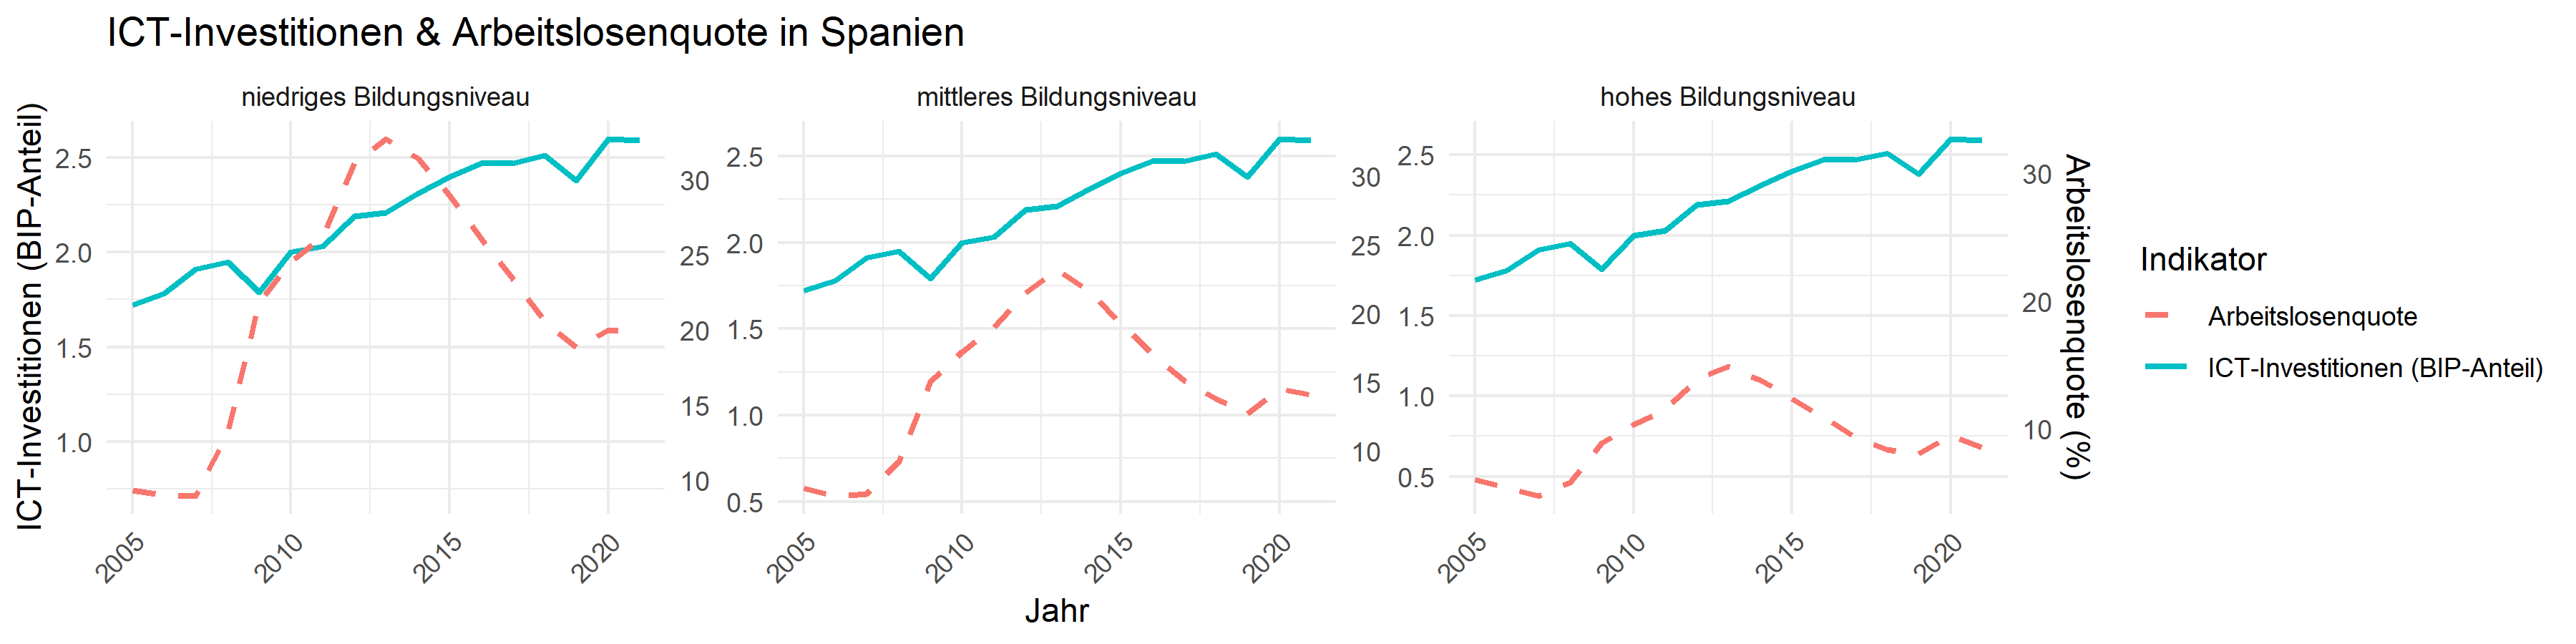
\includegraphics[width=\textwidth]{assets/plot_spain.png}
    \caption{Überblick über \textit{\ac{ICT}-Investitionen} und Arbeitslosenquote in 
    Spanien}
    \label{fig:spain}
\end{figure}

Die Abbildung zeigt die Entwicklung der \textit{\ac{ICT}-Investitionen} als Anteil am 
BIP sowie die Arbeitslosenquote in Spanien zwischen 2005 und 2022, differenziert nach 
Bildungsniveau - Spanien steht hier repräsentativ für südeuropäische Wohlfahrtsstaaten. 
Am Beispiel Spaniens ist ein besonders markanter Anstieg der Arbeitslosenquote während 
der Finanz- und Wirtschaftskrise von 2008 bis 2013 zu beobachten. Während die 
\textit{\ac{ICT}-Investitionen} einen insgesamt moderaten Anstieg über den gesamten 
Zeitraum hinweg zeigen, lassen sich drastische Schwankungen in der Arbeitslosenquote 
identifizieren, insbesondere bei Personen mit niedrigem und mittlerem Bildungsniveau.

Bei Personen mit einem niedrigen Bildungsniveau zeigt sich zwischen 2005 und 2008 
eine relativ stabile Arbeitslosenquote von knapp unter 10\%. Ab 2008 kam es jedoch zu 
einem rasanten Anstieg, der bis 2013 einen Höchststand von über 30\% erreichte. Erst 
nach 2013 begann ein kontinuierlicher Rückgang, der sich bis 2020 auf etwa 20\% 
fortsetzte, bevor ein erneuter leichter Anstieg zu beobachten ist. Die 
\textit{\ac{ICT}-Investitionen} entwickelten sich hingegen gleichmäßiger. Sie begannen 
auf einem niedrigen Niveau von etwa 1,75\% des BIP, zeigten nach der Finanzkriese ab 
2010 eine Aufwärtstendenz und stabilisierten sich nach 2015 bei etwa 2,5\%. Der 
Rückgang der Arbeitslosenquote nach 2013 verlief jedoch unabhängig von einer abrupten 
Zunahme der \textit{\ac{ICT}-Investitionen}, was darauf hindeutet, dass 
makroökonomische Faktoren (z. B. wirtschaftliche Erholung, Beschäftigungsprogramme) 
für die Senkung der Arbeitslosigkeit eine zentrale Rolle spielten.

Bei Personen mit mittlerem Bildungsniveau zeigt sich ein sehr ähnlicher Verlauf. Die 
Arbeitslosenquote lag 2005 noch unter 8\%, stieg im Zuge der Wirtschaftskrise bis 2013 
jedoch auf über 20\% an. Erst ab 2014 begann ein deutlicher Rückgang, der sich bis 
2020 auf etwa 10\% fortsetzte. Die \textit{\ac{ICT}-Investitionen} folgten hier einem 
vergleichbaren Muster wie in der Gruppe der gering Qualifizierten, wobei ein leichter, 
aber kontinuierlicher Anstieg sichtbar ist. Dennoch ist keine direkte Korrelation 
zwischen dem Verlauf der \textit{\ac{ICT}-Investitionen} und der Arbeitslosenquote 
ersichtlich, da der massive Anstieg und der spätere Rückgang der Arbeitslosigkeit 
primär durch die wirtschaftliche Entwicklung und nicht durch technologische 
Investitionen bedingt zu sein scheinen.

Bei Personen mit hohem Bildungsniveau war die Arbeitslosenquote insgesamt niedriger, 
zeigte jedoch ebenfalls einen deutlichen Anstieg während der Wirtschaftskrise. Im Jahr 
2005 lag sie unter 5\%, erreichte 2013 jedoch fast 15\%. Danach setzte auch hier ein 
Rückgang ein, und bis 2020 fiel die Quote auf etwa 5\% zurück. Im Gegensatz zu den 
anderen Bildungsgruppen scheinen sich hier die \textit{\ac{ICT}-Investitionen} und 
die Arbeitslosenquote teilweise gegenläufig zu entwickeln. Während die 
\textit{\ac{ICT}-Investitionen} nach 2010 eine stetige Steigerung zeigen und nach 
2015 stabil auf etwa 2,5\% des BIP bleiben, geht die Arbeitslosenquote in derselben 
Phase zurück. Dies könnte darauf hindeuten, dass hochqualifizierte Arbeitskräfte in 
Spanien stärker von der Digitalisierung profitieren konnten als Personen mit 
niedrigerem Bildungsstand.

Spanien als südeuropäischer Wohlfahrtsstaat ist durch einen stark segmentierten 
Arbeitsmarkt gekennzeichnet, der sich durch hohe Anteile an befristeten 
Beschäftigungsverhältnissen sowie eine geringere Arbeitsplatzsicherheit auszeichnet. 
Dies könnte eine Erklärung für die starken Schwankungen der Arbeitslosenquote 
im Zuge der Finanzkrise sein, da insbesondere gering und mittel Qualifizierte 
von Entlassungen betroffen waren. Die \textit{\ac{ICT}-Investitionen} scheinen 
langfristig zwar leicht anzusteigen, doch zeigt sich kein direkter Zusammenhang 
zwischen diesen Investitionen und der Arbeitslosenquote in den jeweiligen 
Bildungsgruppen. Vielmehr deutet die Entwicklung darauf hin, dass der Arbeitsmarkt 
in Spanien stark konjunkturabhängig ist und die wirtschaftliche Erholung nach 2013 
die wichtigste Triebkraft für die Reduktion der Arbeitslosigkeit war.

Zusammenfassend zeigen die Daten für Spanien eine enge Verbindung zwischen der 
Finanzkrise und den massiven Schwankungen der Arbeitslosenquote, insbesondere bei 
gering und mittel Qualifizierten. Während \textit{\ac{ICT}-Investitionen} über den 
Zeitraum hinweg einen kontinuierlichen, aber moderaten Anstieg zeigen, sind ihre 
direkten Auswirkungen auf die Arbeitslosigkeit unklar. Es könnte jedoch sein, dass 
insbesondere Hochqualifizierte von den steigenden \textit{\ac{ICT}-Investitionen} 
profitieren konnten, während gering Qualifizierte eher von konjunkturellen 
Faktoren abhängig waren.

% Deskriptive Analyse: Grafik "Polen"
\begin{figure}[htbp]
    \centering
    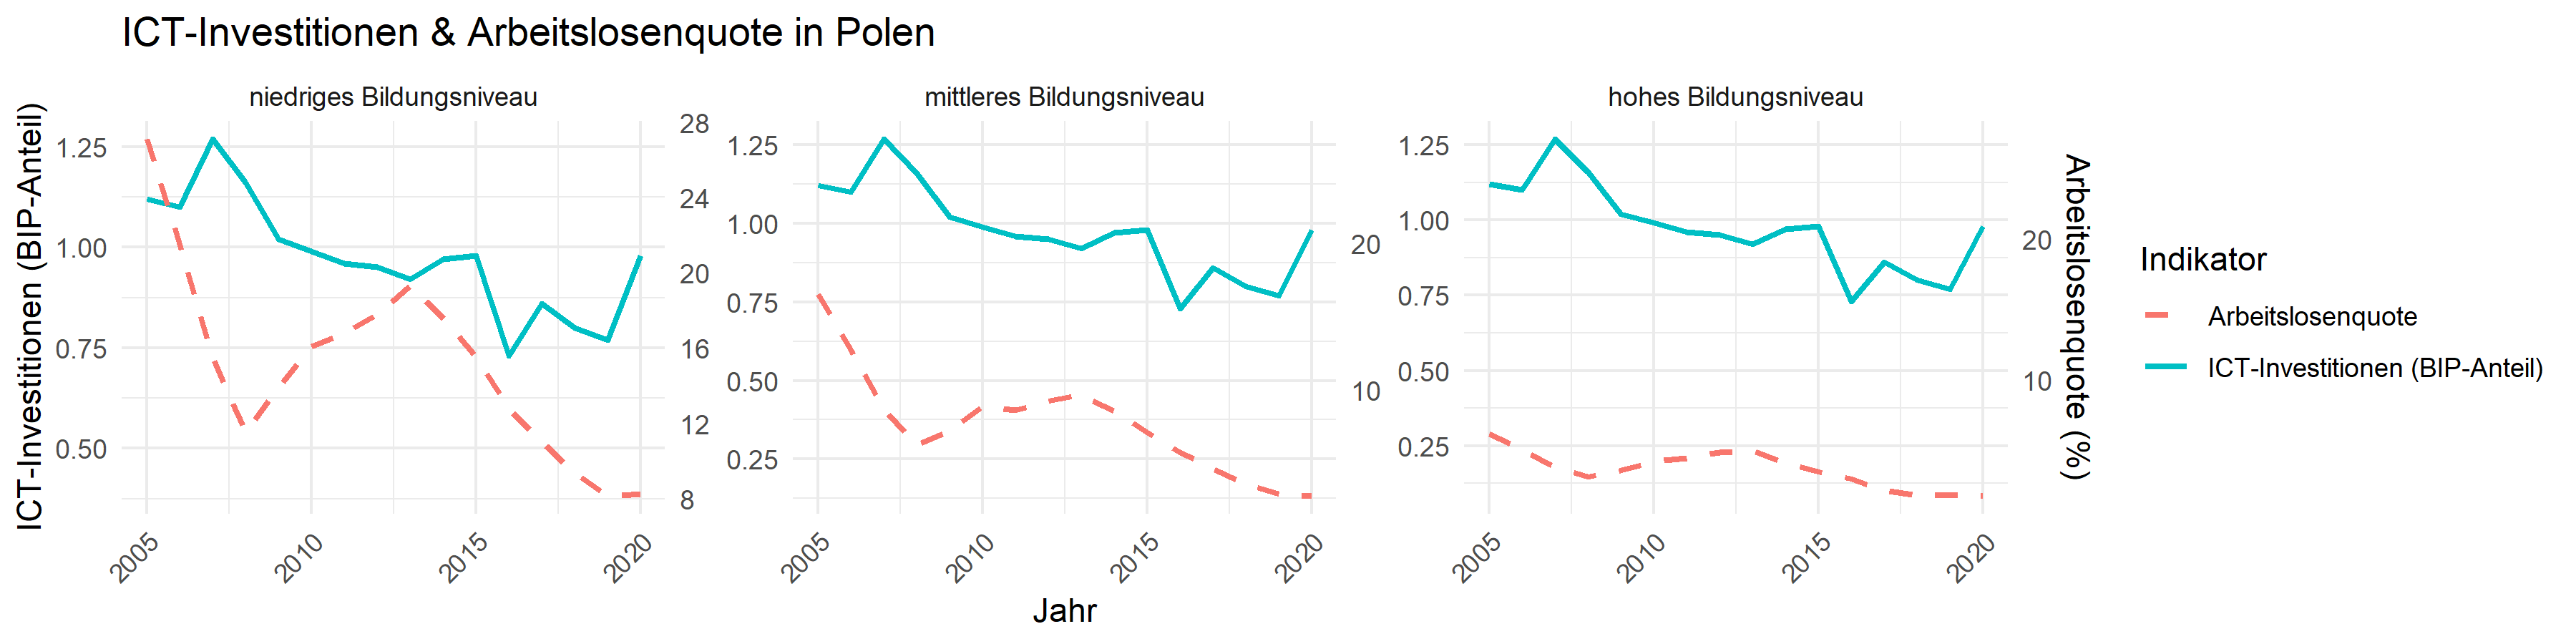
\includegraphics[width=\textwidth]{assets/plot_poland.png}
    \caption{Überblick über \textit{\ac{ICT}-Investitionen} und Arbeitslosenquote 
    in Polen}
    \label{fig:poland}
\end{figure}

Die Abbildung zeigt die Entwicklung der \textit{\ac{ICT}-Investitionen} als Anteil 
am BIP sowie die Arbeitslosenquote in Polen zwischen 2005 und 2022 differenziert 
nach Bildungsniveau - Polen steht hier repräsentativ für postsozialistische 
Wohlfahrtsstaaten.

Auffällig ist der durchgängige Rückgang der Arbeitslosenquote in allen 
Bildungsgruppen, während die \textit{\ac{ICT}-Investitionen} über weite Strecken 
konstant bleiben, beziehungsweise sogar ebenfalls einen Rückgang verzeichnen. Dies 
deutet darauf hin, dass makroökonomische oder arbeitsmarktpolitische Faktoren für 
den Rückgang der Arbeitslosigkeit maßgeblich verantwortlich sein könnten.

Bei Personen mit einem niedrigen Bildungsniveau lag die Arbeitslosenquote im Jahr 
2005 bei knapp 28\%. In den darauffolgenden Jahren kam es zu einem raschen Rückgang, 
wobei jedoch zwischen 2010 und 2015 eine Stagnation mit einem kurzen Anstieg auf fast 
20\% zu beobachten ist. Nach 2015 setzte sich der Rückgang der Arbeitslosenquote 
fort, sodass sie bis 2020 auf 8\% fiel. Die \textit{\ac{ICT}-Investitionen} blieben 
über den gesamten Zeitraum hinweg weitgehend konstant und bewegten sich um die 1\% des 
BIP, mit einem leichten Rückgang zwischen 2010 und 2015. Dies deutet darauf hin, dass  
der starke Rückgang der Arbeitslosigkeit nicht direkt mit den 
\textit{\ac{ICT}-Investitionen} zusammenhängt, sondern durch andere wirtschaftliche 
Faktoren beeinflusst wurde, beispielsweise durch eine allgemeine wirtschaftliche 
Stabilisierung nach dem EU-Beitritt Polens und steigende Beschäftigungsmöglichkeiten 
in arbeitsintensiven Branchen.

Für Personen mit einem mittleren Bildungsniveau zeigt sich ein ähnliches Muster, wenn 
auch auf einem insgesamt niedrigeren Ausgangsniveau der Arbeitslosenquote. Während 
diese 2005 noch über 10\% lag, sank sie in den darauffolgenden Jahren rasch auf etwa 
3\% bis 2015 und weiter unter 2\% bis 2020. Zwischen 2010 und 2015 ist jedoch eine 
leichte Erhöhung der Arbeitslosenquote erkennbar, bevor der Trend weiter nach unten 
verlief. Der Rückgang der Arbeitslosigkeit erfolgt weitgehend unabhängig von der 
Entwicklung der \textit{\ac{ICT}-Investitionen}, was darauf hindeutet, dass 
makroökonomische Faktoren wie die Industrialisierung und eine steigende Nachfrage 
nach Arbeitskräften mit mittlerer Qualifikation eine bedeutendere Rolle gespielt 
haben könnten.

Für Personen mit einem hohen Bildungsniveau war die Arbeitslosenquote bereits 
2005 relativ niedrig, lag aber dennoch bei etwa 6\%, was im Vergleich zu anderen 
europäischen Ländern eher hoch ist. Dies könnte auf strukturelle Faktoren des 
polnischen Arbeitsmarktes zurückzuführen sein, wie eine geringere Anzahl 
hochqualifizierter Beschäftigungsmöglichkeiten in den frühen 2000er-Jahren. In den 
darauffolgenden Jahren fiel die Arbeitslosenquote jedoch deutlich und lag bereits 
2015 unter 2\%. Auffällig ist, dass die \textit{\ac{ICT}-Investitionen} in dieser 
Gruppe im Gegensatz zu den anderen Bildungsgruppen eine leichte Steigerung zeigen. 
In der ersten Hälfte des Beobachtungszeitraums bewegten sich die 
\textit{\ac{ICT}-Investitionen} um 1,2\% des BIP, während sie in den Jahren nach 
2015 tendenziell anstiegen. Dies könnte darauf hindeuten, dass der polnische 
Arbeitsmarkt mit steigendem ICT-Investitionsanteil zunehmend hochqualifizierte 
Beschäftigungsmöglichkeiten geschaffen hat. Dennoch bleibt die Kausalität unklar, 
da die Arbeitslosenquote in dieser Gruppe bereits gefallen war, bevor der leichte 
Anstieg der \textit{\ac{ICT}-Investitionen} einsetzte.

Polen als postsozialistischer Wohlfahrtsstaat hat in den letzten Jahrzehnten einen 
tiefgreifenden wirtschaftlichen Wandel durchlaufen. Der EU-Beitritt im Jahr 2004 
führte zu verstärkten ausländischen Direktinvestitionen, einer zunehmenden 
Integration in europäische Produktionsnetzwerke sowie einer generellen 
Modernisierung der Wirtschaft. Diese Entwicklungen spiegeln sich auch in der 
Reduktion der Arbeitslosigkeit wider, die in allen Bildungsgruppen signifikant 
gesunken ist. Besonders bei Personen mit mittlerem und niedrigem Bildungsniveau 
könnte die Expansion von Industriejobs sowie der Dienstleistungssektor eine 
wesentliche Rolle gespielt haben. % TODO: Zitieren!

Insgesamt zeigt die Abbildung, dass die Arbeitslosenquote in allen Bildungsgruppen 
stark gesunken ist, während die \textit{\ac{ICT}-Investitionen} nur moderate 
Schwankungen aufweisen. Dies deutet darauf hin, dass die Haupttreiber der 
Beschäftigungsentwicklung in Polen eher in wirtschaftlichen und 
arbeitsmarktpolitischen Veränderungen zu suchen sind als in den direkten 
Auswirkungen von \textit{\ac{ICT}-Investitionen}. Dennoch könnte die leichte 
Zunahme der \textit{\ac{ICT}-Investitionen} im späteren Beobachtungszeitraum 
darauf hinweisen, dass sich der polnische Arbeitsmarkt allmählich in Richtung 
einer wissensbasierten Wirtschaft entwickelt, in der besonders Hochqualifizierte 
profitieren.

% Deskriptive Analyse: Grafik "Schweden"
\begin{figure}[htbp]
    \centering
    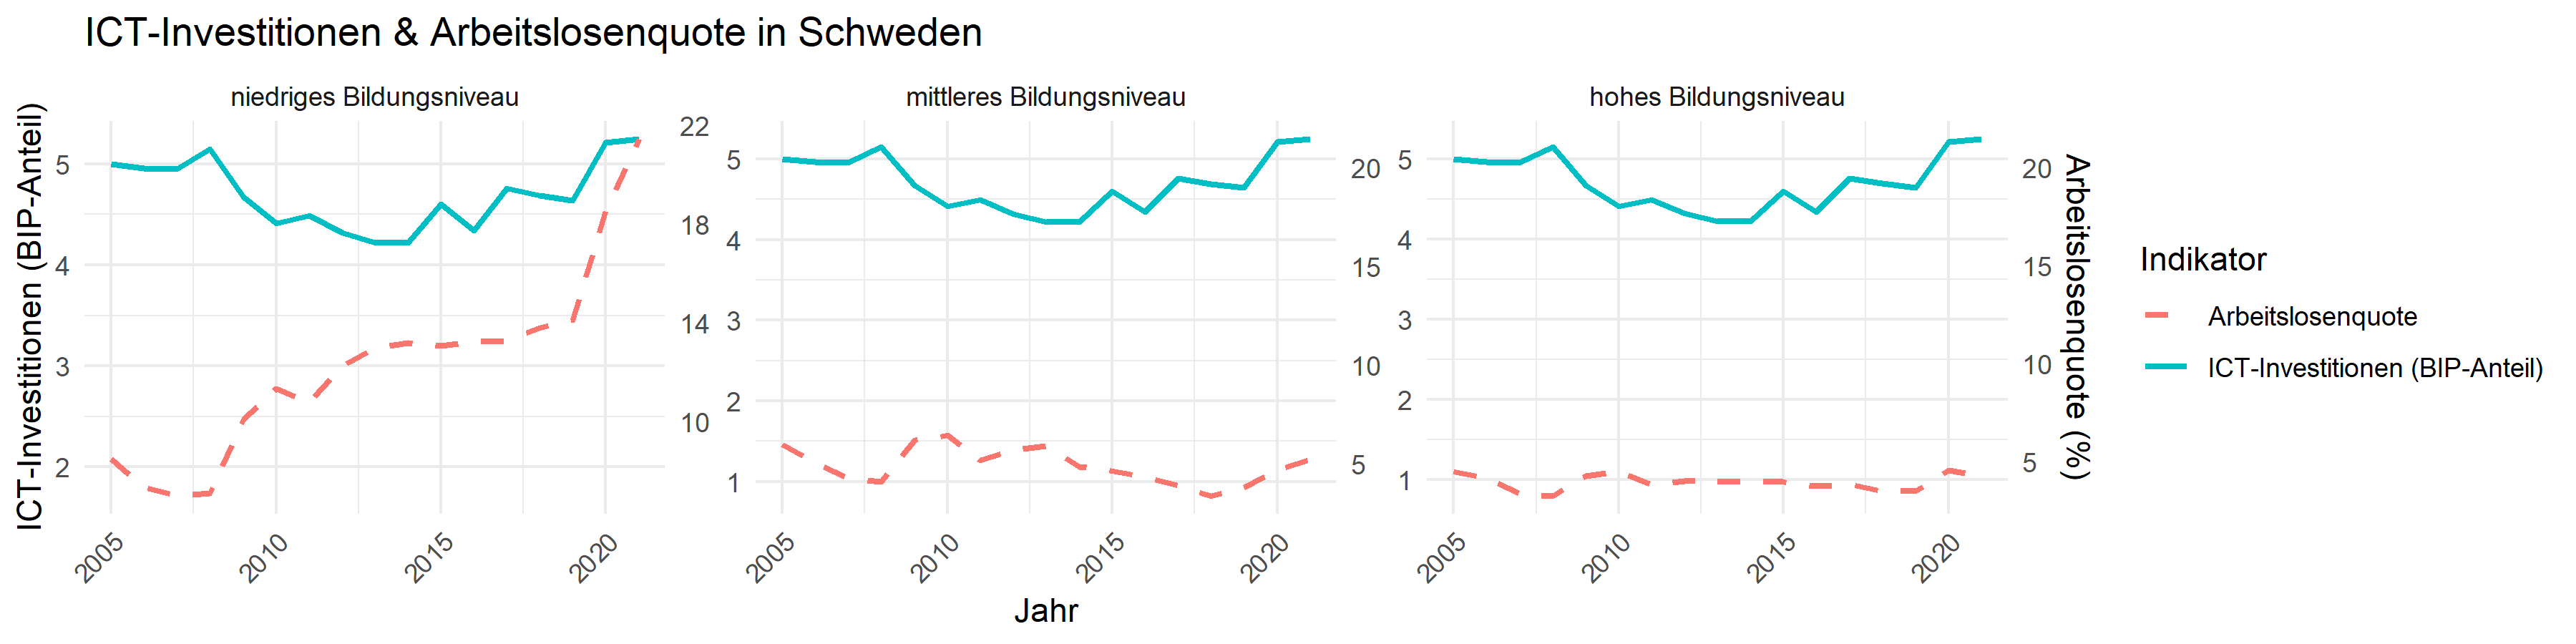
\includegraphics[width=\textwidth]{assets/plot_sweden.png}
    \caption{Überblick über \textit{\ac{ICT}-Investitionen} und Arbeitslosenquote in 
    Schweden}
    \label{fig:sweden}
\end{figure}

Die Abbildung zeigt die Entwicklung der \textit{\ac{ICT}-Investitionen} als Anteil 
am BIP sowie die Arbeitslosenquote in Schweden zwischen 2005 und 2022, differenziert 
nach Bildungsniveau - Schweden steht hier repräsentativ für nordische 
Wohlfahrtsstaaten. Im Gegensatz zu anderen Ländern ist hier eine relativ stabile 
Entwicklung der Arbeitslosenquote über den gesamten Zeitraum zu beobachten, mit nur 
moderaten Schwankungen. Auffällig ist zudem, dass die \textit{\ac{ICT}-Investitionen} 
in Schweden im internationalen Vergleich auf einem vergleichsweise hohen Niveau liegen. 
Während sie in der ersten Dekade leichte Schwankungen zeigen, bleibt ihr Niveau ab 
2010 weitgehend konstant und steigt gegen Ende des Betrachtungszeitraums leicht an.

Bei Personen mit einem niedrigen Bildungsniveau lag die Arbeitslosenquote 2005 bei knapp 
5\% und zeigte bis etwa 2010 einen moderaten Anstieg. Nach 2010 stabilisierte sich die 
Arbeitslosenquote zunächst, bevor sie ab 2015 einen erneuten Aufwärtstrend verzeichnete. 
Besonders auffällig ist der deutliche Anstieg nach 2018, der sich bis 2022 fortsetzt. 
Während die Arbeitslosenquote für gering Qualifizierte also in den letzten Jahren 
gestiegen ist, sind die \textit{\ac{ICT}-Investitionen} im selben Zeitraum weitgehend 
stabil geblieben, wenn auch mit einer leicht positiven Tendenz. Dies könnte darauf 
hindeuten, dass die fortschreitende Digitalisierung möglicherweise die 
Beschäftigungsmöglichkeiten für niedrig qualifizierte Arbeitskräfte verschlechtert hat, 
indem sie bestimmte Arbeitsplätze verdrängte oder die Anforderungen an digitale 
Kompetenzen erhöhte - wahrscheinlich hängt diese Beobachtung aber eher mit der 
Corona-Pandemie zusammen.

Für Personen mit einem mittleren Bildungsniveau zeigt sich ein stabiles Muster, mit 
einer weitgehend konstanten Arbeitslosenquote zwischen 2005 und 2018. Während die 
Arbeitslosigkeit 2005 bei unter 5\% lag, gab es bis 2015 eine leichte Abwärtsbewegung, 
gefolgt von einer weitgehenden Stabilisierung. Nach 2018 zeigt sich eine leicht steigende 
Tendenz der Arbeitslosenquote, wenn auch weniger ausgeprägt als bei den gering 
Qualifizierten. Die \textit{\ac{ICT}-Investitionen} sind in dieser Gruppe durchgängig 
hoch und zeigen eine stabile Entwicklung mit leichten Schwankungen. Anders als bei den 
gering Qualifizierten ist hier keine klare gegenläufige Entwicklung zwischen 
\textit{\ac{ICT}-Investitionen} und Arbeitslosigkeit zu erkennen, was darauf hindeutet, 
dass mittlere Qualifikationen in Schweden weniger stark von den technologischen 
Veränderungen betroffen sind.

Bei Personen mit einem hohen Bildungsniveau zeigt sich über den gesamten Zeitraum 
hinweg eine extrem niedrige Arbeitslosenquote. Bereits 2005 lag sie unter 5\% und blieb 
über den gesamten Zeitraum stabil, mit nur minimalen Schwankungen. Auffällig ist, dass 
die \textit{\ac{ICT}-Investitionen} in dieser Gruppe im internationalen Vergleich sehr 
hoch sind, mit Werten, die konstant bei 4-5\% des \ac{BIP} liegen. Die Kombination aus 
hoher \ac{ICT}-Investition und niedriger Arbeitslosenquote deutet darauf hin, dass 
hochqualifizierte Arbeitskräfte in Schweden stark von der Digitalisierung profitieren 
konnten. Dies entspricht auch theoretischen Erwartungen, da hochqualifizierte 
Beschäftigte in wissensintensiven Branchen tätig sind, die von technologischen 
Innovationen profitieren.

Schweden als nordischer Wohlfahrtsstaat zeichnet sich durch ein stark reguliertes, 
aber flexibles Arbeitsmarktsystem aus, das durch hohe Sozialleistungen, eine starke 
Gewerkschaftsbindung und ein gut ausgebautes Bildungssystem geprägt ist. Die stabilen 
\textit{\ac{ICT}-Investitionen} und die insgesamt niedrigen Arbeitslosenquoten deuten 
darauf hin, dass der schwedische Arbeitsmarkt relativ widerstandsfähig gegenüber 
technologischen Veränderungen ist. Allerdings lässt sich bei niedrig qualifizierten 
Arbeitskräften ein Anstieg der Arbeitslosigkeit nach 2018 beobachten, der 
möglicherweise mit strukturellen Veränderungen auf dem Arbeitsmarkt zusammenhängt. 
Dies könnte darauf hindeuten, dass bestimmte Berufe durch die Digitalisierung 
zunehmend verdrängt werden oder dass sich die Anforderungen an digitale Kompetenzen 
verstärkt haben, sodass Geringqualifizierte Schwierigkeiten haben, sich an die 
veränderten Bedingungen anzupassen.

Insgesamt zeigt die Abbildung, dass Schweden ein stabiles Beschäftigungsniveau über 
den gesamten Zeitraum hinweg aufweist, wobei die \textit{\ac{ICT}-Investitionen} 
konstant hoch sind. Während Hoch- und Mittelqualifizierte weitgehend von den 
Entwicklungen profitieren konnten, scheint sich für gering Qualifizierte in den 
letzten Jahren eine Verschlechterung der Beschäftigungssituation abzuzeichnen. Dies 
könnte darauf hindeuten, dass Digitalisierung in hochentwickelten Volkswirtschaften 
wie Schweden zunehmend zu einer Polarisierung des Arbeitsmarktes führt, bei der 
Hochqualifizierte von den Investitionen profitieren, während gering Qualifizierte 
zunehmend unter Druck geraten.

% Deskriptive Analyse: Grafik "Deutschland"
\begin{figure}[htbp]
    \centering
    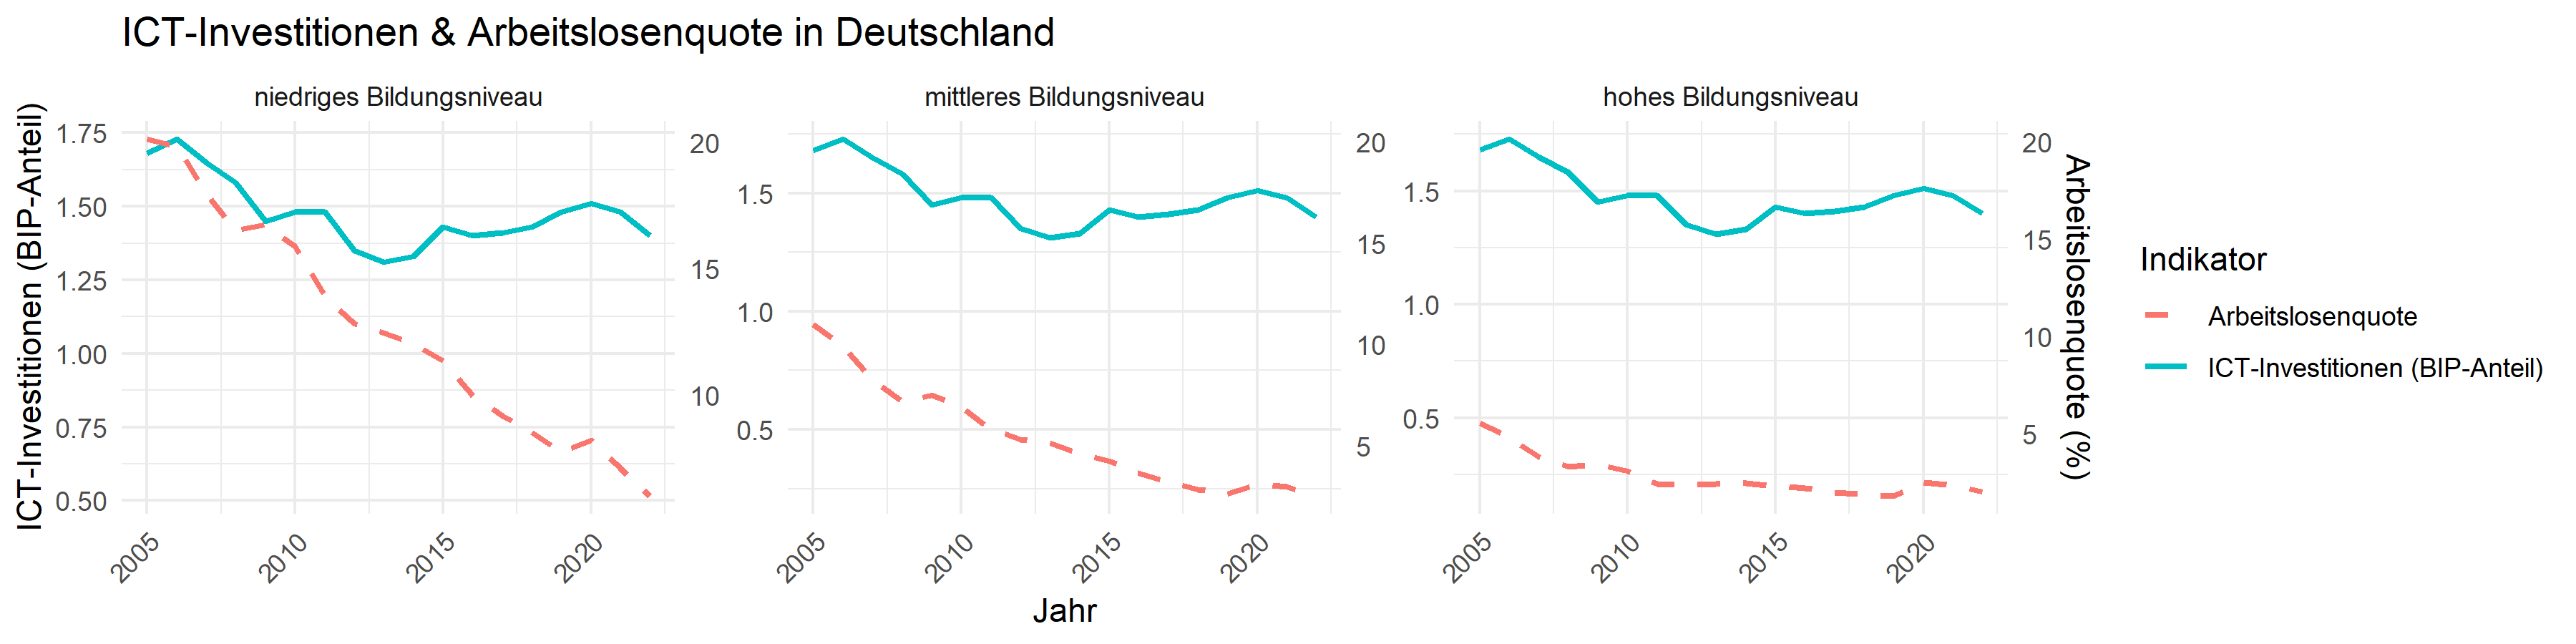
\includegraphics[width=\textwidth]{assets/plot_germany.png}
    \caption{Überblick über \textit{\ac{ICT}-Investitionen} und Arbeitslosenquote in 
    Deutschland}
    \label{fig:germany}
\end{figure}

Die Abbildung zeigt die Entwicklung der \textit{\ac{ICT}-Investitionen} als Anteil 
am BIP sowie die Arbeitslosenquote in Deutschland zwischen 2005 und 2022, 
differenziert nach Bildungsniveau - Deutschland steht hier repräsentativ für 
mitteleuropäische Wohlfahrtsstaaten. Dabei lassen sich klare Unterschiede zwischen 
den drei betrachteten Gruppen - niedriges, mittleres und hohes Bildungsniveau - sowohl 
hinsichtlich des Niveaus als auch der Veränderung der Arbeitslosenquoten erkennen. 
Insgesamt zeigen sich über den gesamten Zeitraum hinweg deutliche Rückgänge in der 
Arbeitslosenquote, während die \textit{\ac{ICT}-Investitionen} eine weitgehend 
stabile Entwicklung aufweisen.

Für Personen mit einem niedrigen Bildungsniveau zeigt sich eine besonders hohe 
Arbeitslosenquote zu Beginn des Beobachtungszeitraums, die 2005 bei über 18\% lag. 
In den darauffolgenden Jahren kam es zu einem kontinuierlichen Rückgang, der bis 2020 
Werte unter 5\% erreichte. Diese Entwicklung spiegelt die allgemeine Verbesserung des 
deutschen Arbeitsmarktes wider, insbesondere durch wirtschaftlichen Aufschwung und 
Reformen im Rahmen der Agenda 2010. Die \textit{\ac{ICT}-Investitionen} verzeichneten 
zwischen 2005 und 2010 zunächst einen leichten Rückgang, bevor sie sich um die 1,5\% 
des BIP stabilisierten. Ein direkter Zusammenhang zwischen 
\textit{\ac{ICT}-Investitionen} und der sinkenden Arbeitslosenquote ist nicht 
ersichtlich, da der Rückgang der Arbeitslosenquote bereits vor der leichten 
Stabilisierung der Investitionen begann.

Bei Personen mit mittlerem Bildungsniveau zeigt sich ein ähnliches Muster, wenn auch 
auf einem insgesamt niedrigeren Ausgangsniveau der Arbeitslosenquote. Während diese 
2005 noch bei etwa 10\% lag, fiel sie bis 2020 auf rund 3\% und blieb seither 
weitgehend stabil. Die \textit{\ac{ICT}-Investitionen} zeigen eine konstante 
Entwicklung mit geringen Schwankungen. Auch hier bleibt der direkte Zusammenhang 
zwischen den \textit{\ac{ICT}-Investitionen} und der Arbeitslosenquote unklar, da 
der Rückgang der Arbeitslosigkeit langfristig verläuft und nicht direkt mit den 
Investitionen korreliert.

Für Personen mit hohem Bildungsniveau zeigt sich über den gesamten Zeitraum hinweg 
eine sehr niedrige Arbeitslosenquote. Bereits 2005 lag sie unter 5\% und sank bis
 2010 auf unter 2\%, wo sie anschließend auf diesem niedrigen Niveau stabil blieb. 
 Im Vergleich zu den anderen Bildungsgruppen weist diese Gruppe somit die geringsten 
 Schwankungen auf. Die \textit{\ac{ICT}-Investitionen} zeigen auch hier eine 
 weitgehend stabile Entwicklung. Dies könnte darauf hindeuten, dass Hochqualifizierte 
 vermehrt in Berufen tätig sind, die von steigenden \textit{\ac{ICT}-Investitionen} 
 profitieren, jedoch bleibt auch hier die Kausalität unklar.

Deutschland als konservativer Wohlfahrtsstaat zeichnet sich durch eine enge Verzahnung 
von Bildungssystem und Arbeitsmarkt aus. Insbesondere das duale Ausbildungssystem 
und gezielte arbeitsmarktpolitische Maßnahmen könnten eine Rolle beim Rückgang der 
Arbeitslosenquoten in den niedrigen und mittleren Bildungsgruppen gespielt haben. 
Die \textit{\ac{ICT}-Investitionen} zeigen über den Beobachtungszeitraum hinweg keine 
drastischen Veränderungen, was darauf hindeutet, dass technologische Entwicklungen 
schrittweise in den Arbeitsmarkt integriert wurden. Besonders für Hochqualifizierte 
könnte eine steigende Nachfrage nach digitalen Fähigkeiten eine Rolle gespielt 
haben, während bei den niedrigen und mittleren Bildungsniveaus der 
Arbeitsmarktrückgang vermutlich durch andere makroökonomische Faktoren beeinflusst 
wurde.

Die Abbildung verdeutlicht insgesamt, dass die Arbeitslosenquoten in allen 
Bildungsgruppen über die Jahre hinweg gesunken sind, während die 
\textit{\ac{ICT}-Investitionen} vergleichsweise stabil geblieben sind. Dies lässt darauf 
schließen, dass der Rückgang der Arbeitslosigkeit nicht direkt durch 
\textit{\ac{ICT}-Investitionen} getrieben wurde, sondern eher mit makroökonomischen 
Entwicklungen und strukturellen Veränderungen auf dem deutschen Arbeitsmarkt 
zusammenhängt.

% Deskriptive Analyse: Grafik "Großbritannien"
\begin{figure}[htbp]
    \centering
    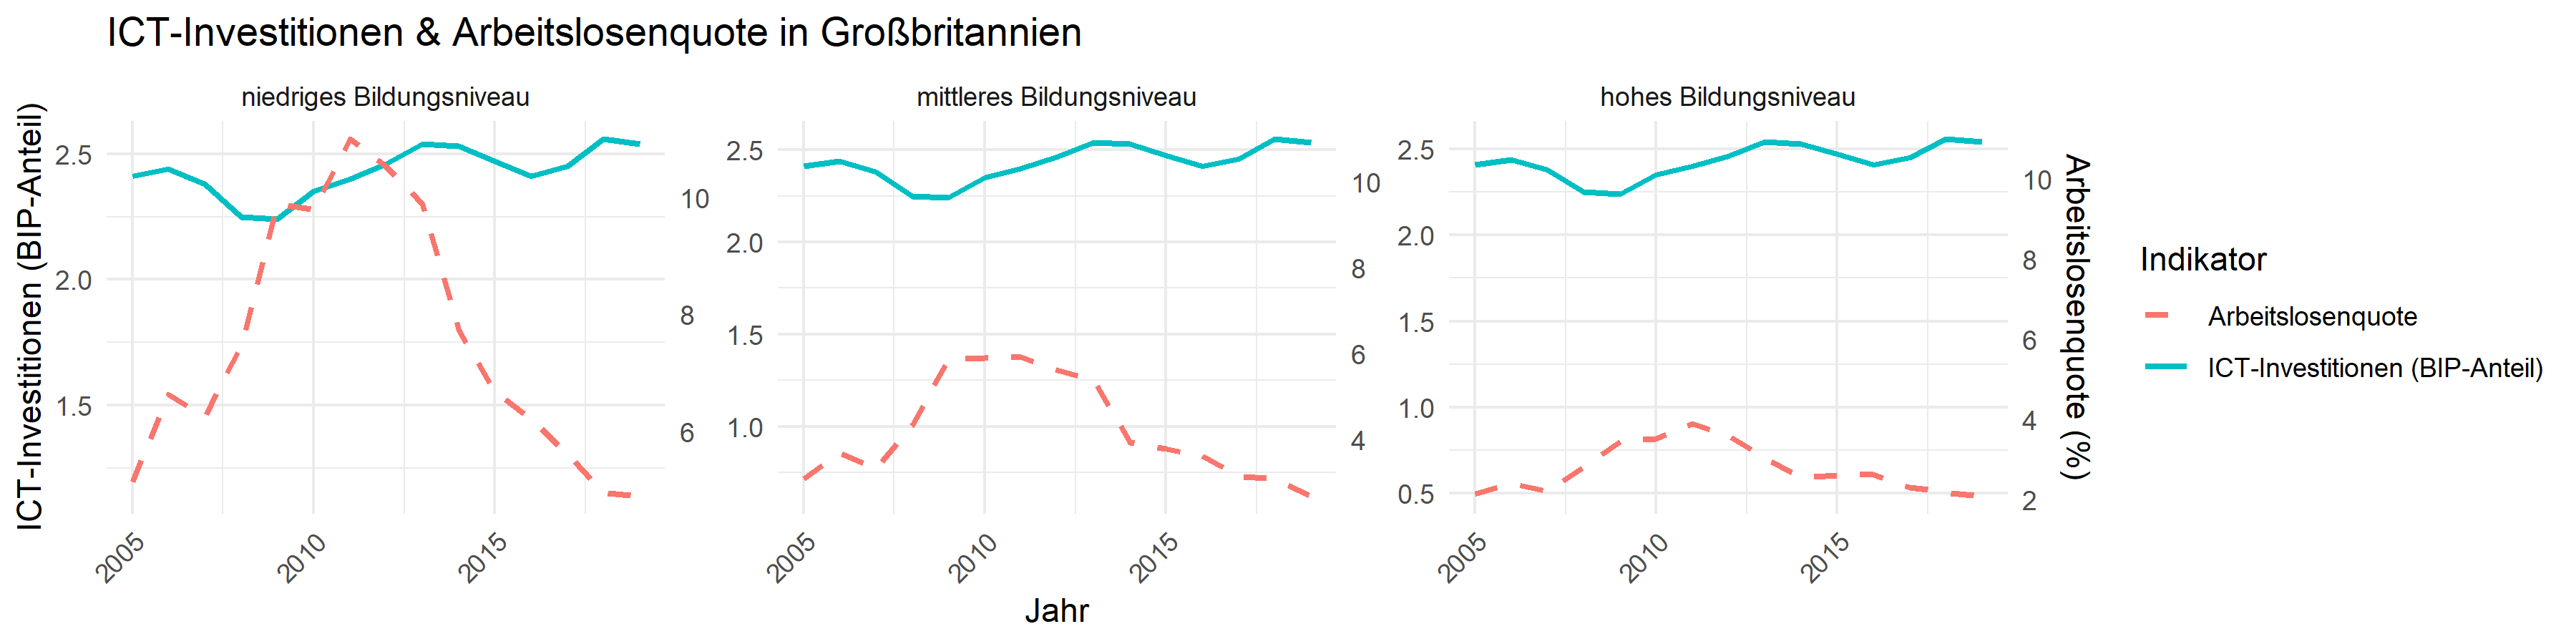
\includegraphics[width=\textwidth]{assets/plot_uk.png}
    \caption{Überblick über \textit{\ac{ICT}-Investitionen} und Arbeitslosenquote in 
    Großbritannien}
    \label{fig:uk}
\end{figure}

Die Abbildung zeigt die Entwicklung der \textit{\ac{ICT}-Investitionen} als Anteil am BIP 
sowie die Arbeitslosenquote in Großbritannien zwischen 2005 und 2022, differenziert nach 
Bildungsniveau - Großbritannien steht hier repräsentativ für angelsächsische 
Wohlfahrtsstaaten. Im Vergleich zu anderen Wohlfahrtsstaatentypen weist Großbritannien eine 
relativ konstante Arbeitslosenquote auf, die über den Zeitraum hinweg nur leichte 
Rückgänge zeigt. Auffällig ist, dass die \textit{\ac{ICT}-Investitionen} in Großbritannien 
zwar einen moderaten Anstieg aufweisen, sich jedoch auf einem relativ niedrigen Niveau 
bewegen.

Bei Personen mit einem niedrigen Bildungsniveau lag die Arbeitslosenquote im Jahr 2005 
bei etwa 8\% und sank bis 2020 auf unter 4\%. Anders als in Ländern mit stärker 
regulierten Arbeitsmärkten zeigt sich hier kein abrupter Rückgang, sondern eine 
schrittweise Anpassung über den Zeitraum hinweg. Gleichzeitig zeigen die 
\textit{\ac{ICT}-Investitionen} einen leicht steigenden Trend, bleiben jedoch im Bereich 
von etwa 1,5\% des BIP. Ein klarer Zusammenhang zwischen \textit{\ac{ICT}-Investitionen} 
und der Arbeitslosenquote lässt sich nicht unmittelbar erkennen, was darauf hindeuten 
könnte, dass andere arbeitsmarktpolitische oder wirtschaftliche Faktoren maßgeblicher für 
die Reduktion der Arbeitslosigkeit sind.

Bei Personen mit mittlerem Bildungsniveau zeigt sich ein ähnliches Muster. Die 
Arbeitslosenquote lag 2005 bei etwa 6\% und fiel bis 2015 auf rund 3\%, wo sie sich 
anschließend stabilisierte. Die \textit{\ac{ICT}-Investitionen} zeigen hier eine geringe 
Zunahme, bleiben jedoch weitgehend konstant im Bereich von 1,5\% bis 2\% des BIP. Auch in 
dieser Gruppe scheint der Rückgang der Arbeitslosenquote eher mit marktwirtschaftlichen 
Anpassungen als mit direkten Effekten der \textit{\ac{ICT}-Investitionen} zusammenzuhängen. 
Der relativ geringe Anstieg der Investitionen deutet darauf hin, dass die britische 
Wirtschaft zwar technologische Entwicklungen integriert, jedoch nicht in dem Ausmaß wie 
andere hochdigitalisierte Volkswirtschaften.

Für Personen mit hohem Bildungsniveau zeigt sich über den gesamten Zeitraum hinweg eine 
sehr niedrige Arbeitslosenquote. Bereits 2005 lag sie unter 3\% und blieb über den 
gesamten Zeitraum weitgehend stabil, mit nur minimalen Schwankungen. Die 
\textit{\ac{ICT}-Investitionen} zeigen auch hier eine relativ konstante Entwicklung, 
liegen jedoch ebenfalls im Bereich von 1,5\% bis 2\% des BIP. Dies deutet darauf hin, 
dass Hochqualifizierte kaum von negativen Beschäftigungseffekten durch Digitalisierung 
betroffen sind. Vielmehr könnte der flexible britische Arbeitsmarkt es dieser Gruppe 
erleichtert haben, sich an technologische Veränderungen anzupassen.

Großbritannien als anglo-sächsischer Wohlfahrtsstaat zeichnet sich durch einen 
weniger regulierten Arbeitsmarkt aus, der sich durch eine hohe Flexibilität und eine 
geringere staatliche Intervention auszeichnet. Diese Charakteristik könnte erklären, 
warum die Arbeitslosenquoten über den Zeitraum hinweg relativ stabil bleiben und 
gleichzeitig keine drastischen Veränderungen im Bereich der \textit{\ac{ICT}-Investitionen} 
feststellbar sind. Der moderate Rückgang der Arbeitslosigkeit deutet darauf hin, dass sich 
der britische Arbeitsmarkt schrittweise an Digitalisierung angepasst hat, ohne dass 
bestimmte Gruppen massiv benachteiligt wurden.

Zusammenfassend zeigt die Abbildung, dass sich die britische Arbeitslosenquote über die 
Jahre hinweg in allen Bildungsgruppen verringert hat, wenn auch nicht so drastisch wie in 
anderen Ländern. Gleichzeitig bleiben die \textit{\ac{ICT}-Investitionen} auf einem 
relativ niedrigen Niveau und zeigen keine unmittelbare Korrelation mit den Veränderungen 
der Arbeitslosenquote. Dies deutet darauf hin, dass makroökonomische Faktoren wie die 
Arbeitsmarktflexibilität und allgemeine wirtschaftliche Entwicklung eine wichtigere Rolle 
für die Beschäftigungsdynamik spielen als allein die Höhe der \textit{\ac{ICT}-Investitionen}.


%%%%%%%%%%%%%%%%%%%%%%%%%
% Multivariate Analysen %
%%%%%%%%%%%%%%%%%%%%%%%%%

\subsection{Multivariate Analysen}

% Multivariate Analyse: Einleitung
Die Zusammenfassung der Ergebnisse aus den Modellen mit Kontrollvariablen zeigt eine 
umfassende, jedoch differenzierte Analyse der Auswirkungen von 
\textit{\ac{ICT}-Investitionen} auf die Arbeitslosenquote in den drei Bildungsgruppen 
(„niedriges Bildungsniveau“, „mittleres Bildungsniveau“, „hohes Bildungsniveau“). Die 
Modelle liefern wichtige Hinweise auf die Bedeutung makroökonomischer Rahmenbedingungen 
und institutioneller Strukturen, während der direkte Einfluss von 
\textit{\ac{ICT}-Investitionen} weniger eindeutig ist.

% Multivariate Analyse: Modelle ohne Interaktion/Jahres-Dummy
\begin{table}[H]
\resizebox{\textwidth}{!}{
\centering
\begin{talltblr}[         %% tabularray outer open
entry=none,label=none,
note{}={+ p \num{< 0.1}, * p \num{< 0.05}, ** p \num{< 0.01}, *** p \num{< 0.001}},
]                     %% tabularray outer close
{                     %% tabularray inner open
colspec={Q[]Q[]Q[]Q[]},
column{2,3,4}={}{halign=c,},
column{1}={}{halign=l,},
hline{8}={1,2,3,4}{solid, black, 0.05em},
}                     %% tabularray inner close
\toprule
& niedriges
Bildungsniv.
(Kontrolle) & mittleres
Bildungsniv.
(Kontrolle) & hohes
Bildungsniv.
(Kontrolle) \\ \midrule %% TinyTableHeader
ICT\_INVEST\_SHARE\_GDP & \num{-0.323}  & \num{-0.116}  & \num{-0.057}  \\
& (\num{0.554}) & (\num{0.338}) & (\num{0.187}) \\
GDP\_PER\_CAPITA         & \num{0.000}+  & \num{0.000}*  & \num{0.000}   \\
& (\num{0.000}) & (\num{0.000}) & (\num{0.000}) \\
PERCENT\_EMPLOYEES\_TUD  & \num{0.011}   & \num{0.032}   & \num{-0.026}  \\
& (\num{0.111}) & (\num{0.068}) & (\num{0.037}) \\
Num.Obs.                   & \num{502}     & \num{502}     & \num{502}     \\
R2                         & \num{0.019}   & \num{0.025}   & \num{0.007}   \\
R2 Adj.                    & \num{-0.048}  & \num{-0.042}  & \num{-0.061}  \\
AIC                        & \num{2948.8}  & \num{2453.8}  & \num{1860.6}  \\
BIC                        & \num{2965.6}  & \num{2470.6}  & \num{1877.5}  \\
RMSE                       & \num{4.53}    & \num{2.77}    & \num{1.53}    \\
\bottomrule
\end{talltblr}
}
\caption{Einzelwerte der Regressionsmodellparameter für die Kontrollmodelle}
\label{tab:models_control}
\end{table}


% Multivariate Analyse: Modell ohne Interaktion/Jahres-Dummy (niedriges Bildungsniveau)
Im Modell für die Gruppe mit niedrigem Bildungsniveau zeigt der geschätzte Koeffizient 
für \textit{\ac{ICT}-Investitionen} einen positiven Wert von 0.572, der jedoch statistisch 
nicht signifikant ist. Dies deutet darauf hin, dass \textit{\ac{ICT}-Investitionen} 
keinen systematischen Einfluss auf die Arbeitslosenquote dieser Gruppe haben, da die 
Ergebnisse keine klare Richtung oder signifikante Kausalität nahelegen.

Das \textit{\ac{BIP} pro Kopf} zeigt mit einem Koeffizienten von -0.120 (p < 0.05) einen 
negativen und signifikanten Einfluss. Dies weist darauf hin, dass in wohlhabenderen 
Ländern die Arbeitslosenquote für geringqualifizierte Personen tendenziell niedriger ist, 
möglicherweise aufgrund eines breiteren Angebots an Beschäftigungsmöglichkeiten oder 
arbeitsmarktpolitischer Maßnahmen.

Die \textit{Gewerkschaftsdichte} weist mit einem Koeffizienten von 0.136 einen leicht 
positiven, aber statistisch nicht signifikanten Zusammenhang auf. Dies deutet darauf 
hin, dass eine höhere gewerkschaftliche Organisationsrate möglicherweise mit einer 
leicht höheren Arbeitslosenquote für diese Gruppe einhergeht, dieser Effekt jedoch 
nicht robust genug ist, um als signifikant zu gelten.

% Multivariate Analyse: Modell ohne Interaktion/Jahres-Dummy (mittleres Bildungsniveau)
Für das mittlere Bildungsniveau ergibt sich ein leicht positives Bild. Der geschätzte 
Koeffizient für \textit{\ac{ICT}-Investitionen} beträgt 0.377, ist jedoch statistisch 
nicht signifikant. Dies deutet darauf hin, dass \textit{\ac{ICT}-Investitionen} keinen 
direkten Einfluss auf die Arbeitslosenquote dieser Gruppe haben, während andere nicht 
modellierte Faktoren möglicherweise eine größere Rolle spielen.

Das \textit{\ac{BIP} pro Kopf} zeigt mit einem Koeffizienten von -0.097 (p < 0.01) einen 
signifikant negativen Zusammenhang. Dies deutet darauf hin, dass eine höhere 
Wirtschaftsleistung mit einer geringeren Arbeitslosenquote für mittelqualifizierte Personen 
verbunden ist. Diese Beobachtung widerspricht der ursprünglichen Annahme eines positiven 
Zusammenhangs und legt nahe, dass wirtschaftlich stärkere Länder bessere 
Beschäftigungsmöglichkeiten für diese Gruppe bieten.

Die \textit{Gewerkschaftsdichte} weist mit einem Koeffizienten von 0.131 einen leicht 
positiven Zusammenhang auf (p < 0.1), was darauf hindeuten könnte, dass eine stärkere 
gewerkschaftliche Organisation möglicherweise mit leicht erhöhten Arbeitslosenquoten 
für diese Gruppe einhergeht. Der Effekt bleibt jedoch nur schwach signifikant.

% Multivariate Analyse: Modell ohne Interaktion/Jahres-Dummy (hohes Bildungsniveau)
Für das hohe Bildungsniveau zeigt das Modell mit einem Koeffizienten von 0.154 den schwächsten 
positiven Zusammenhang zwischen \textit{\ac{ICT}-Investitionen} und der Arbeitslosenquote. 
Dieser Wert ist jedoch statistisch nicht signifikant, was darauf hindeutet, dass 
\textit{\ac{ICT}-Investitionen} keinen systematischen Einfluss auf die Arbeitslosigkeit von 
Hochqualifizierten haben. Dies könnte darauf hinweisen, dass hochqualifizierte Arbeitskräfte 
sich flexibler an die Anforderungen des digitalen Arbeitsmarkts anpassen können, sodass der 
direkte Einfluss von \textit{\ac{ICT}-Investitionen} in dieser Gruppe geringer ausfällt.

Das \textit{\ac{BIP} pro Kopf} zeigt mit einem Koeffizienten von -0.050 (p < 0.01) einen 
signifikant negativen Zusammenhang, was darauf hindeutet, dass eine höhere Wirtschaftsleistung 
in einem Land mit einer geringeren Arbeitslosenquote für Hochqualifizierte verbunden ist. 
Dies widerspricht der ursprünglichen Annahme, dass makroökonomische Unterschiede in Ländern 
mit höherem Bildungsniveau eine geringere Rolle für die Arbeitsmarktsituation von 
Hochqualifizierten spielen.

Die \textit{Gewerkschaftsdichte} hat in dieser Gruppe einen leicht positiven Effekt (0.040), 
bleibt jedoch statistisch insignifikant. Dies könnte darauf hindeuten, dass hochqualifizierte 
Arbeitskräfte weniger von institutionellen Faktoren wie gewerkschaftlicher Organisation 
abhängig sind.

% Modellgüte und Interpretation der Ergebnisse
Die Modellgüte variiert zwischen den Bildungsgruppen, wobei die erklärten Varianzen (R²-Werte) 
höher als zuvor, aber weiterhin moderat bleiben. Im Modell für das niedrige Bildungsniveau 
beträgt der R²-Wert 0.272, für das mittlere Bildungsniveau 0.301 und für das hohe 
Bildungsniveau 0.276. Diese Werte zeigen, dass die Modelle einen relevanten, aber begrenzten 
Anteil der Variation in der Arbeitslosenquote erklären können. Dennoch bleibt ein großer Teil 
der Variabilität durch nicht berücksichtigte Faktoren unbeeinflusst.

Der adjustierte R²-Wert liegt bei 0.193 (niedriges Bildungsniveau), 0.226 (mittleres 
Bildungsniveau) und 0.198 (hohes Bildungsniveau). Diese Werte sind zwar positiv, aber dennoch 
vergleichsweise niedrig. Dies deutet darauf hin, dass weitere wesentliche Einflussfaktoren in 
dieser Analyse nicht berücksichtigt wurden. Insbesondere branchenspezifische Entwicklungen, 
individuelle Qualifikationsmaßnahmen oder regionale Unterschiede könnten wichtige 
Erklärungsgrößen sein, die in den Modellen nicht erfasst wurden.

% Fazit der multivariaten Analyse ohne Interaktion
Zusammenfassend zeigen die Modelle mit Kontrollvariablen, dass \textit{\ac{ICT}-Investitionen} 
in keiner Bildungsgruppe einen signifikanten Einfluss auf die Arbeitslosenquote haben. Die 
geschätzten Koeffizienten sind durchweg niedrig (niedriges Bildungsniveau: 0.572, mittleres 
Bildungsniveau: 0.377, hohes Bildungsniveau: 0.154) und statistisch nicht signifikant. Dies 
deutet darauf hin, dass Investitionen in digitale Technologien allein keine klaren Effekte 
auf die Arbeitslosenquote zeigen, sondern dass weitere Faktoren eine Rolle spielen.

Dagegen zeigt sich, dass makroökonomische Faktoren, insbesondere das \textit{\ac{BIP} pro 
Kopf}, in allen Modellen einen signifikanten Einfluss auf die Arbeitslosenquote haben. In 
allen Bildungsgruppen sind die Koeffizienten für das \textit{\ac{BIP} pro Kopf} negativ und 
signifikant (niedriges Bildungsniveau: -0.120, mittleres Bildungsniveau: -0.097*, hohes 
Bildungsniveau: -0.050**). Dies deutet darauf hin, dass höhere wirtschaftliche Entwicklung mit 
einer tendenziell niedrigeren Arbeitslosenquote einhergeht – möglicherweise, weil wohlhabendere 
Länder mehr Möglichkeiten zur Arbeitsmarktintegration bieten oder strukturelle Arbeitslosigkeit 
besser abfedern können.

Die Erklärungswerte (R²) der Modelle sind moderat (zwischen 0.272 und 0.301), was darauf 
hindeutet, dass ein Teil der Variation in der Arbeitslosenquote durch die berücksichtigten 
Faktoren erklärt wird, aber weiterhin wesentliche strukturelle und institutionelle 
Einflussfaktoren fehlen. Dies zeigt die Notwendigkeit einer differenzierteren Untersuchung, 
insbesondere durch Interaktionsmodelle, um institutionelle Rahmenbedingungen besser zu verstehen 
und die Mechanismen hinter den beobachteten Zusammenhängen genauer zu erfassen.

% Multivariate Analyse: Modelle mit Interaktion & Jahres-Dummy
\begin{table}[H]
\resizebox{\textwidth}{!}{ % Resize to fit the page width
\centering
\begin{talltblr}[         %% tabularray outer open
entry=none,label=none,
note{}={+ p \num{< 0.1}, * p \num{< 0.05}, ** p \num{< 0.01}, *** p \num{< 0.001}},
]                     %% tabularray outer close
{                     %% tabularray inner open
colspec={Q[]Q[]Q[]Q[]},
column{2,3,4}={}{halign=c,},
column{1}={}{halign=l,},
hline{50}={1,2,3,4}{solid, black, 0.05em},
}                     %% tabularray inner close
\toprule
& niedriges
Bildungsniv.
(Interaktion) & mittleres
Bildungsniv.
(Interaktion) & hohes
Bildungsniv.
(Interaktion) \\ \midrule %% TinyTableHeader
ICT\_INVEST\_SHARE\_GDP                                    & \num{3.899}*   & \num{2.817}**  & \num{1.132}*   \\
& (\num{1.664})  & (\num{1.007})  & (\num{0.563})  \\
YEAR\_FACTOR2006                                             & \num{-0.634}   & \num{-0.397}   & \num{-0.252}   \\
& (\num{1.049})  & (\num{0.635})  & (\num{0.355})  \\
YEAR\_FACTOR2007                                             & \num{-1.606}   & \num{-0.891}   & \num{-0.383}   \\
& (\num{1.080})  & (\num{0.654})  & (\num{0.366})  \\
YEAR\_FACTOR2008                                             & \num{-1.330}   & \num{-0.622}   & \num{-0.344}   \\
& (\num{1.115})  & (\num{0.675})  & (\num{0.377})  \\
YEAR\_FACTOR2009                                             & \num{2.750}*   & \num{2.045}**  & \num{0.900}*   \\
& (\num{1.081})  & (\num{0.654})  & (\num{0.366})  \\
YEAR\_FACTOR2010                                             & \num{4.503}*** & \num{3.328}*** & \num{1.635}*** \\
& (\num{1.104})  & (\num{0.668})  & (\num{0.374})  \\
YEAR\_FACTOR2011                                             & \num{4.627}*** & \num{3.080}*** & \num{1.652}*** \\
& (\num{1.134})  & (\num{0.686})  & (\num{0.384})  \\
YEAR\_FACTOR2012                                             & \num{5.531}*** & \num{3.713}*** & \num{2.034}*** \\
& (\num{1.158})  & (\num{0.701})  & (\num{0.392})  \\
YEAR\_FACTOR2013                                             & \num{5.795}*** & \num{4.065}*** & \num{2.381}*** \\
& (\num{1.199})  & (\num{0.727})  & (\num{0.406})  \\
YEAR\_FACTOR2014                                             & \num{4.796}*** & \num{3.624}*** & \num{2.169}*** \\
& (\num{1.236})  & (\num{0.748})  & (\num{0.418})  \\
YEAR\_FACTOR2015                                             & \num{3.897}**  & \num{3.121}*** & \num{1.997}*** \\
& (\num{1.298})  & (\num{0.786})  & (\num{0.440})  \\
YEAR\_FACTOR2016                                             & \num{4.158}**  & \num{3.408}*** & \num{2.021}*** \\
& (\num{1.393})  & (\num{0.844})  & (\num{0.472})  \\
YEAR\_FACTOR2017                                             & \num{1.637}    & \num{1.997}*   & \num{1.257}*   \\
& (\num{1.476})  & (\num{0.894})  & (\num{0.500})  \\
YEAR\_FACTOR2018                                             & \num{0.456}    & \num{1.399}    & \num{1.035}+   \\
& (\num{1.564})  & (\num{0.947})  & (\num{0.529})  \\
YEAR\_FACTOR2019                                             & \num{0.196}    & \num{1.328}    & \num{1.001}+   \\
& (\num{1.678})  & (\num{1.017})  & (\num{0.568})  \\
YEAR\_FACTOR2020                                             & \num{1.197}    & \num{2.168}*   & \num{1.723}**  \\
& (\num{1.723})  & (\num{1.044})  & (\num{0.583})  \\
YEAR\_FACTOR2021                                             & \num{2.532}    & \num{2.872}*   & \num{1.870}**  \\
& (\num{1.946})  & (\num{1.179})  & (\num{0.659})  \\
YEAR\_FACTOR2022                                             & \num{2.088}    & \num{2.823}*   & \num{1.778}*   \\
& (\num{2.326})  & (\num{1.409})  & (\num{0.788})  \\
GDP\_PER\_CAPITA                                            & \num{0.000}*   & \num{0.000}**  & \num{0.000}**  \\
& (\num{0.000})  & (\num{0.000})  & (\num{0.000})  \\
PERCENT\_EMPLOYEES\_TUD                                     & \num{0.074}    & \num{0.102}    & \num{0.025}    \\
& (\num{0.104})  & (\num{0.063})  & (\num{0.035})  \\
ICT\_INVEST\_SHARE\_GDP × WELFARE\_STATECentral European  & \num{-0.152}   & \num{-1.075}   & \num{-0.491}   \\
& (\num{2.020})  & (\num{1.223})  & (\num{0.684})  \\
ICT\_INVEST\_SHARE\_GDP × WELFARE\_STATENordic            & \num{0.582}    & \num{-0.653}   & \num{0.271}    \\
& (\num{2.336})  & (\num{1.415})  & (\num{0.791})  \\
ICT\_INVEST\_SHARE\_GDP × WELFARE\_STATEPost-socialist    & \num{-4.817}** & \num{-3.163}** & \num{-1.252}*  \\
& (\num{1.751})  & (\num{1.060})  & (\num{0.593})  \\
ICT\_INVEST\_SHARE\_GDP × WELFARE\_STATESouthern European & \num{0.605}    & \num{-2.433}   & \num{-2.737}** \\
& (\num{3.022})  & (\num{1.830})  & (\num{1.023})  \\
Num.Obs.                                                      & \num{502}      & \num{502}      & \num{502}      \\
R2                                                            & \num{0.312}    & \num{0.328}    & \num{0.303}    \\
R2 Adj.                                                       & \num{0.231}    & \num{0.248}    & \num{0.220}    \\
AIC                                                           & \num{2812.3}   & \num{2308.7}   & \num{1725.1}   \\
BIC                                                           & \num{2917.8}   & \num{2414.2}   & \num{1830.6}   \\
RMSE                                                          & \num{3.79}     & \num{2.30}     & \num{1.28}     \\
\bottomrule
\end{talltblr}
}
\caption{Einzelwerte der Regressionsmodellparameter für die Interaktionsmodelle}
\label{tab:models_interaction}
\end{table}


% Multivariate Analyse mit Interaktion und Jahres-Dummies
Die Modelle mit Interaktionseffekten und Jahresdummies liefern eine differenziertere Perspektive 
auf den Zusammenhang zwischen \textit{\ac{ICT}-Investitionen} und der Arbeitslosenquote. Im 
Gegensatz zu den Basis-Modellen ohne Interaktionen zeigen sich hier mehrere signifikante 
Zusammenhänge, insbesondere mit institutionellen Faktoren wie dem Wohlfahrtsstaatentyp.

% Haupteffekte von ICT-Investitionen
Der geschätzte Haupteffekt von \textit{\ac{ICT}-Investitionen} ist in allen drei 
Bildungsgruppen positiv und signifikant. Für das niedrige Bildungsniveau zeigt sich mit einem 
Koeffizienten von +3.899 (p < 0.05) ein deutlicher Anstieg der Arbeitslosenquote bei 
höheren ICT-Investitionen. Auch für das mittlere Bildungsniveau ist der Effekt mit 
+2.817 (p < 0.01) signifikant positiv. Beim hohen Bildungsniveau ist der Effekt mit 
+1.132 (p < 0.05) zwar schwächer ausgeprägt, aber weiterhin signifikant.

Diese Ergebnisse deuten darauf hin, dass höhere ICT-Investitionen in angelsächsischen 
Wohlfahrtsstaaten (Referenzkategorie) mit einer höheren Arbeitslosenquote in allen 
Bildungsgruppen verbunden sind.

Dies könnte darauf hinweisen, dass die Flexibilität des liberalen Arbeitsmarktes allein nicht 
ausreicht, um negative Beschäftigungseffekte durch die Digitalisierung abzufedern. 
Während Digitalisierung häufig mit Effizienzsteigerungen verbunden wird, könnten Automatisierung 
und technologische Substitution insbesondere niedrig- und mittelqualifizierte Arbeitskräfte 
stärker betreffen.

% Interaktionseffekte zwischen ICT-Investitionen und Wohlfahrtsstaaten
Die Interaktionseffekte zwischen \textit{\ac{ICT}-Investitionen} und den 
Wohlfahrtsstaaten liefern wichtige Erkenntnisse über die Rolle institutioneller 
Rahmenbedingungen. Hierbei ist nochmals zu erwähnen, dass für die Analyse "anglosächsisch" 
als Referenzkategorie gewählt wurde - die Ergebnisse sind relativ zu dieser Kategorie zu 
interpretieren:

\begin{itemize}
    \item \textbf{Postsozialistische Wohlfahrtsstaaten:} Hier zeigen sich 
    die stärksten negativen Effekte. Für das niedrige Bildungsniveau beträgt der 
    Interaktionseffekt -4.817 (p < 0.01), für das mittlere Bildungsniveau -3.163 (p < 0.01) und 
    für das hohe Bildungsniveau -1.252 (p < 0.05). Diese signifikant negativen Werte 
    deuten darauf hin, dass ICT-Investitionen in diesen Ländern keine positiven Effekte 
    auf die Arbeitsmarktsituation haben, sondern möglicherweise bestehende 
    strukturelle Schwächen verschärfen. Eine mögliche Erklärung hierfür ist, dass die 
    Digitalisierung in diesen Ländern schneller voranschreitet als die institutionellen 
    Anpassungen im Bildungssystem und am Arbeitsmarkt.
    
    \item \textbf{Mitteleuropäische Wohlfahrtsstaaten:} Der Interaktionseffekt ist für alle 
    Bildungsgruppen negativ, aber nicht signifikant. Dies deutet darauf hin, dass 
    ICT-Investitionen hier keinen starken moderierenden Einfluss auf die Arbeitslosigkeit 
    haben. Mitteleuropäische Länder wie Deutschland oder Frankreich verfügen über 
    duale Bildungssysteme und relativ stabile Arbeitsmarktstrukturen, die mögliche 
    negative Effekte von ICT-Investitionen abmildern könnten.
    
    \item \textbf{Nordische Wohlfahrtsstaaten:} Hier zeigen sich ebenfalls keine signifikanten 
    Interaktionseffekte. Die Ergebnisse deuten darauf hin, dass nordische Länder besser 
    auf die digitale Transformation vorbereitet sind und ICT-Investitionen nicht mit 
    steigender Arbeitslosigkeit verbunden sind.
    
    \item \textbf{Südeuropäische Wohlfahrtsstaaten:} Für das niedrige und mittlere Bildungsniveau 
    sind die Interaktionseffekte nicht signifikant. Im hohen Bildungsniveau ist der 
    Interaktionseffekt jedoch -2.737 (p < 0.01) und damit stark negativ. Dies deutet 
    darauf hin, dass selbst hochqualifizierte Arbeitskräfte in diesen Ländern durch 
    strukturelle Arbeitsmarktprobleme benachteiligt sind und ICT-Investitionen hier eher 
    bestehende Ungleichheiten verstärken, anstatt sie zu verringern.
\end{itemize}

% Modellgüte und Vergleich mit den Basis-Modellen
Die erklärten Varianzen (R²-Werte) sind in den Interaktionsmodellen deutlich höher als in 
den Basis-Modellen ohne Interaktionen. Während die R²-Werte in den einfachen Modellen 
zwischen 0.019 und 0.025 lagen, erreichen die Interaktionsmodelle Werte von 0.312 
(niedriges Bildungsniveau), 0.328 (mittleres Bildungsniveau) und 0.303 (hohes Bildungsniveau). 
Dies zeigt, dass institutionelle Rahmenbedingungen eine wesentliche Rolle spielen und die 
Erklärungskraft der Modelle erheblich verbessern.

Der adjustierte R²-Wert bleibt zwar mit 0.231–0.248 weiterhin vergleichsweise niedrig, 
aber deutlich höher als in den Kontrollmodellen. Dies unterstreicht, dass die reine 
Betrachtung von ICT-Investitionen ohne Berücksichtigung institutioneller Faktoren keine 
adäquate Erklärung für Unterschiede in den Arbeitslosenquoten liefert.

% Fazit der Modelle mit Interaktion und Jahresdummies
Zusammenfassend zeigen die Modelle mit Interaktionseffekten, dass der Einfluss von 
\textit{\ac{ICT}-Investitionen} auf die Arbeitslosenquote stark von den institutionellen 
Rahmenbedingungen abhängt. Während die Basiswerte der ICT-Investitionen in allen 
Bildungsgruppen positiv sind, deuten die Interaktionseffekte darauf hin, dass insbesondere 
postsozialistische und südeuropäische Wohlfahrtsstaaten größere Schwierigkeiten haben, 
die positiven Effekte der Digitalisierung für den Arbeitsmarkt zu nutzen. 

Besonders in postsozialistischen Ländern könnte dies auf eine Diskrepanz zwischen 
Digitalisierungsfortschritt und institutioneller Anpassungsfähigkeit zurückzuführen sein. 
Die Ergebnisse zeigen, dass eine starke wirtschaftliche Basis allein nicht ausreicht, um 
die Herausforderungen der digitalen Transformation zu bewältigen. Vielmehr müssen 
gezielte politische Maßnahmen ergriffen werden, um Bildungs- und Arbeitsmarktsysteme auf 
die neuen Anforderungen anzupassen.

Die Kombination aus ICT-Investitionen, institutionellen Rahmenbedingungen und 
makroökonomischen Faktoren bestimmt maßgeblich, wie sich die Digitalisierung auf 
Arbeitsmärkte auswirkt. Während in gut funktionierenden Arbeitsmärkten mit starken 
Bildungssystemen (z. B. Nordische Länder) ICT-Investitionen kaum negative Effekte haben, 
sind in Ländern mit weniger flexiblen Arbeitsmärkten (z. B. Südeuropa, 
Postsozialistische Staaten) signifikante Herausforderungen erkennbar.

Die Modelle verdeutlichen somit, dass ICT-Investitionen alleine keine universelle Lösung 
für Arbeitsmarktprobleme darstellen, sondern dass ihre Wirksamkeit stark von den 
institutionellen Gegebenheiten abhängt. Besonders in Ländern mit ineffizienten 
Arbeitsmarktstrukturen und fehlenden Anpassungsmaßnahmen sind Reformen notwendig, um 
die Vorteile der Digitalisierung optimal zu nutzen.

% TODO: Diskussion und Fazit mit neuen Ergebnissen abgleichen...

\section{Diskussion und Fazit}

Die Ergebnisse dieser Arbeit bieten wertvolle Einblicke in die Beziehung zwischen 
\ac{ICT}-Investitionen und der Arbeitslosenquote in verschiedenen Bildungsgruppen. Sie 
zeigen signifikante Zusammenhänge und verdeutlichen die Rolle institutioneller 
Rahmenbedingungen für die Beschäftigungswirkungen der Digitalisierung. Die Untersuchung 
trägt zur wissenschaftlichen Debatte über die Wechselwirkungen zwischen technologischer 
Entwicklung, Arbeitsmarktstrukturen und politischen Institutionen bei und liefert 
praktische Implikationen für Politik, Unternehmen und Bildungssysteme.

\subsection{Zentrale Ergebnisse der Analyse}

Die Analyse zeigt, dass \ac{ICT}-Investitionen über alle Bildungsgruppen hinweg einen 
signifikant positiven Effekt auf die Arbeitslosenquote haben. Dieser Effekt ist für 
gering- und mittelqualifizierte Personen besonders stark ausgeprägt, bleibt aber auch für 
hochqualifizierte Arbeitskräfte signifikant. Dies widerspricht der weit verbreiteten 
Annahme, dass Digitalisierung primär positive Effekte für Hochqualifizierte hat, während 
gering Qualifizierte besonders negativ betroffen sind.

Die Interaktionsmodelle liefern weitere wichtige Erkenntnisse über die Moderationseffekte 
institutioneller Rahmenbedingungen. Besonders in postsozialistischen und südeuropäischen 
Wohlfahrtsstaaten sind die negativen Beschäftigungseffekte von \ac{ICT}-Investitionen am 
stärksten ausgeprägt. Dies deutet darauf hin, dass diese Länder strukturelle Herausforderungen 
bei der Anpassung an technologische Entwicklungen haben, insbesondere in Bezug auf 
Weiterbildungsangebote und arbeitsmarktpolitische Schutzmechanismen.

Die Regulierungsstrenge des Arbeitsmarkts zeigt differenzierte Effekte: Während sie für 
Geringqualifizierte tendenziell negativ wirkt (d. h. strengere Regulierung erhöht die 
Arbeitslosenquote), hat sie für Hochqualifizierte eher stabilisierende Effekte. Der 
Anteil tertiär gebildeter Personen hat in allen Bildungsgruppen einen signifikant 
negativen Einfluss auf die Arbeitslosenquote. Dies deutet darauf hin, dass eine höhere 
Bildungsbeteiligung langfristig dazu beiträgt, negative Beschäftigungseffekte der Digitalisierung 
abzumildern.

Zusammenfassend legen die Ergebnisse nahe, dass die Auswirkungen von Investitionen in \ac{ICT}  
nicht nur durch technologische Faktoren bestimmt werden, sondern maßgeblich von 
wirtschaftlichen, politischen und institutionellen Rahmenbedingungen abhängen. In Ländern 
mit flexibleren Arbeitsmarktstrukturen und besser ausgebauten Weiterbildungssystemen fallen 
die negativen Effekte deutlich schwächer aus als in Ländern mit rigiden Strukturen.

\subsection{Einordnung der Ergebnisse in den theoretischen Kontext}

Die Theorie des \ac{SBTC} besagt, dass technologische Innovationen die Nachfrage nach 
hochqualifizierten Arbeitskräften steigern, während gering Qualifizierte durch 
Automatisierung verdrängt werden \parencite[S. 7]{acemoglu2002technical}. Die Ergebnisse 
dieser Arbeit bestätigen diese Annahme jedoch nur teilweise. Während erwartet wurde, dass 
\ac{ICT}-Investitionen primär die Arbeitslosenquote von gering Qualifizierten erhöhen, 
zeigen die Modelle einen durchweg signifikanten positiven Effekt für alle Bildungsgruppen. 
Das bedeutet, dass die negativen Arbeitsmarkteffekte der Digitalisierung nicht nur auf 
niedrigqualifizierte Arbeitnehmer beschränkt sind, sondern auch mittel- und hochqualifizierte 
Arbeitskräfte betreffen können.

Eine mögliche Erklärung für dieses Ergebnis liegt in der unterschiedlichen Geschwindigkeit 
der Digitalisierung in verschiedenen Branchen. Während einige Industriezweige stark von 
Automatisierung betroffen sind, entstehen gleichzeitig neue Beschäftigungsfelder, insbesondere 
im Bereich digitaler Dienstleistungen und IT-Sektoren \parencite[S. 1554-1555]{autor2013thegrowth}. 
Dies könnte dazu führen, dass die erwartete Polarisierung der Arbeitsmärkte durch 
\ac{ICT}-Investitionen in der Praxis nicht so eindeutig ausfällt, wie es die \ac{SBTC}-Theorie 
prognostiziert.

Die Ergebnisse zeigen zudem, dass institutionelle Rahmenbedingungen eine zentrale Rolle 
für die Anpassung an digitale Transformationsprozesse spielen. Besonders in 
postsozialistischen und südeuropäischen Wohlfahrtsstaaten sind \ac{ICT}-Investitionen mit 
stärkeren negativen Beschäftigungseffekten verbunden. Dies deutet darauf hin, dass diese 
Länder größere Schwierigkeiten haben, die digitalen Transformationsprozesse in ihre 
Arbeitsmarkt- und Bildungssysteme zu integrieren. In nordischen und mitteleuropäischen 
Wohlfahrtsstaaten sind diese Effekte hingegen schwächer ausgeprägt, was darauf hindeutet, 
dass eine stärkere arbeitsmarktpolitische Absicherung und bessere Weiterbildungsangebote 
die negativen Effekte der Digitalisierung abfedern können 
\parencite[S. 27-30]{espingandersen1990thethree}.

\subsection{Limitationen und zukünftige Forschung}

Trotz der wertvollen Erkenntnisse dieser Untersuchung sind einige Limitationen zu 
berücksichtigen. Erstens basiert die Analyse auf aggregierten \ac{OECD}-Daten für den 
Zeitraum 2005–2022, wodurch Unterschiede in der Erhebungsmethodik zwischen den 
Ländern die Ergebnisse potenziell verzerren könnten. Zweitens liegt der Fokus der 
Untersuchung auf makroökonomischen Zusammenhängen. Individuelle Anpassungsstrategien 
von Arbeitnehmer*innen oder Unternehmen an die Digitalisierung konnten in dieser 
Analyse nicht berücksichtigt werden. Künftige Studien sollten daher verstärkt auf 
Umfragedaten oder firmenspezifische Datenquellen zurückgreifen, um differenziertere 
Erkenntnisse zu gewinnen.

Darüber hinaus berücksichtigt die gewählte Fixed-Effects-Panelanalyse keine nicht-linearen 
Zusammenhänge oder dynamischen Anpassungsprozesse. Es wäre sinnvoll, alternative 
Modellansätze wie nicht-lineare Panelmodelle oder differenzierte Zeitreihenanalysen 
zu verwenden, um kausale Mechanismen noch präziser zu identifizieren.

Neben diesen methodischen Einschränkungen ergeben sich aus den Ergebnissen weiterführende 
Forschungsfragen. Insbesondere bleibt offen, welche politischen und wirtschaftlichen 
Mechanismen die Fähigkeit einzelner Länder beeinflussen, ICT-Investitionen erfolgreich in 
den Arbeitsmarkt zu integrieren. Ebenso stellt sich die Frage, welche Rolle Weiterbildung 
und digitale Qualifikationen für die Beschäftigungseffekte von ICT-Investitionen spielen 
und inwiefern branchenspezifische Unterschiede die Auswirkungen der Digitalisierung moderieren.

\subsection{Gesamtfazit}

Zusammenfassend zeigen die Ergebnisse, dass \ac{ICT}-Investitionen keine universelle 
Lösung für Arbeitsmarktprobleme darstellen, sondern dass ihre Wirkungen maßgeblich von 
institutionellen Rahmenbedingungen abhängen. Während in Ländern mit gut entwickelten 
Arbeitsmarkt- und Bildungssystemen die negativen Effekte begrenzt sind, weisen insbesondere 
südeuropäische und postsozialistische Wohlfahrtsstaaten signifikante Herausforderungen auf.

Diese Befunde verdeutlichen, dass eine erfolgreiche digitale Transformation nicht nur von 
technologischen Investitionen abhängt, sondern auch von arbeitsmarktpolitischen, 
wirtschaftlichen und bildungspolitischen Maßnahmen begleitet werden muss. Insbesondere 
Weiterbildungsprogramme, Reformen der Arbeitsmarktregulierungen und gezielte Fördermaßnahmen 
für benachteiligte Gruppen könnten entscheidend dazu beitragen, die positiven Potenziale 
der Digitalisierung zu realisieren und die Risiken einer verstärkten Arbeitsmarktpolarisierung 
zu minimieren.


% Literaturverzeichnis
\printbibliography

\newpage

% Anhang
\appendix
% TODO: Prüfungsleistung unterschreiben!
% TODO: Codebook aktualisieren (am Ende)!

\section{Anhang}

%%%%%%%%%%%%%%%%%%
% Projektdateien %
%%%%%%%%%%%%%%%%%%

\subsection{Projektdateien}

Alle Projektdateien (R-Code, TeX-Dateien, sowie alle Datensätze) welche für die Arbeit und die 
Analyse genutzt wurden, sind gebündelt im folgenden GitHub Repository zu finden (der erste Link 
führt zum Repository - der zweite direkt zum R-Codebook):

\vspace{2cm}

\begin{center}
    
\includegraphics[width=0.3\textwidth]{assets/qrcode_repository.png}\\
    \small\url{https://github.com/TAR-IT/bachelorthesis}
\end{center}

\vspace{2cm}

\begin{center}
    
\includegraphics[width=0.3\textwidth]{assets/qrcode_codebook.png}\\
    \small\url{https://github.com/TAR-IT/bachelorthesis/blob/main/R/codebook.R}
\end{center}
\newpage

%%%%%%%%%%%%%%%%%%%%%%%%%%%%%%%%%%
% Erklärung zur Prüfungsleistung %
%%%%%%%%%%%%%%%%%%%%%%%%%%%%%%%%%%

\subsection{Erklärung zur Prüfungsleistung}

Name, Vorname: Rau, Tobias Achim \\
Matrikelnummer: 6619097 \\
Studiengang: Politikwissenschaften BA

\vspace{0.5cm}

Die am FB03 gültige Definition von Plagiaten ist mir vertraut und verständlich: 

\begin{quote}
    „Eine am FB03 eingereichte Arbeit wird als Plagiat identifiziert, wenn in ihr nachweislich 
    fremdes geistiges Eigentum ohne Kennzeichnung verwendet wird und dadurch dessen Urheberschaft 
    suggeriert oder behauptet wird. Das geistige Eigentum kann ganze Texte, Textteile, 
    Formulierungen, Ideen, Argumente, Abbildungen, Tabellen oder Daten umfassen und muss als 
    geistiges Eigentum der Urheberin/des Urhebers gekennzeichnet sein. Sofern eingereichte 
    Arbeiten die Kennzeichnung vorsätzlich unterlassen, provozieren sie einen Irrtum bei 
    denjenigen, welche die Arbeit bewerten, und erfüllen somit den Tatbestand der Täuschung.“
\end{quote}

Ich versichere hiermit, dass ich die eingereichte Arbeit mit dem Titel 

% Titel der Arbeit
\begin{center}
    \textbf{"\ac{ICT}-Investitionen und Arbeitslosigkeit in Wohlfahrtsstaaten - \\ 
    eine Paneldatenanalyse nach Bildungsniveau in OECD-Ländern"} \\ 
\end{center}

nach den Regeln guter wissenschaftlicher Praxis angefertigt habe. Alle Stellen, die wörtlich oder 
sinngemäß aus Veröffentlichungen oder aus anderen fremden Mitteilungen entnommen wurden, sind als 
solche kenntlich gemacht. Die vorliegende Arbeit ist von mir selbständig und ohne Benutzung 
anderer als der angegebenen Quellen und Hilfsmittel verfasst worden. Ebenfalls versichere ich, 
dass diese Arbeit noch in keinem anderen Modul oder Studiengang als Prüfungsleistung vorgelegt 
wurde.

\vspace{0.5cm}

Mir ist bekannt, dass Plagiate auf Grundlage der Studien- und Prüfungsordnung im Prüfungsamt 
dokumentiert und vom Prüfungsausschuss sanktioniert werden. Diese Sanktionen können neben dem 
Nichtbestehen der Prüfungsleistung weitreichende Folgen bis hin zum Ausschluss von der Erbringung 
weiterer Prüfungsleistungen für mich haben. 

\vfill

\begin{flushleft}
    \small Rödermark, \today,
    % \raisebox{-0.65cm}{\includegraphics[width=0.3\textwidth]{assets/signature.pdf}}
    \\[-0.6cm]
    \_\_\_\_\_\_\_\_\_\_\_\_\_\_\_\_\_\_\_\_\_\_\_\_\_\_\_\_\_\_\_\_\_ \\
    \small\textit{(Ort, Datum, Unterschrift)}
\end{flushleft}



\end{document}
